\chapter{Анализ графов спутников полученных при помощи polaris 2.0}

Для оценки влияния космической погоды на бортовые системы и целевую аппаратуру
малых космических аппаратов (МКА) в этой главе будет проведен комплексный анализ
зависимости параметров телеметрии \cite{green_2017_impact}
\cite{schlag_2018_numerical} \cite{boumghar_2018_enhanced}, индексов солнечной
активности и геомагнитных индексов. В основе исследования лежит применение
модели машинного обучения Polaris ML. Результаты работы модели будут
представлены в виде двухмерного графа связности, отражающего выявленные
взаимосвязи между исследуемыми параметрами.

Для расчета и анализа графа связности будет использована обширная база данных
телеметрии сети наземных станций SatNOGS. Параметры солнечной активности будут
извлечены из следующих основных источников:

\begin{itemize}[wide]
	\item Центр прогнозирования космической погоды (Space Weather Prediction Center, SWPC/SWO) \cite{swpc_noaa_data_souce};
	\item Центр наблюдения и анализа данных о влиянии Солнца в Брюсселе (Solar Influences Data Analysis Center, S.I.D.C.) \cite{silso_snd_data_source};
	\item Канадская радиоастрофизическая обсерватория в Пентиктоне \cite{swgc_flux_data_source}.
\end{itemize}

Далее представлена таблица \ref{tab:detailed_solar_geo_params} с основными анализируемыми параметрами солнечной активности

\begin{longtable}{|l|p{12cm}|}
	\caption{Подробное описание параметров солнечной и геомагнитной активности}
	\label{tab:detailed_solar_geo_params}                                                                                                                                                                                                                                                                                                                                                                                                                                                                                                    \\

	\hline
	\textbf{Параметр}     & \textbf{Описание}                                                                                                                                                                                                                                                                                                                                                                                                                                                                                                \\
	\hline
	\endfirsthead

	\multicolumn{2}{c}%
	{\tablename\ \thetable\ -- \textit{Продолжение}}                                                                                                                                                                                                                                                                                                                                                                                                                                                                                         \\
	\hline
	\textbf{Параметр}     & \textbf{Описание}                                                                                                                                                                                                                                                                                                                                                                                                                                                                                                \\
	\hline
	\endhead

	\hline
	\multicolumn{2}{|r|}{\textit{Продолжение на следующей странице}}                                                                                                                                                                                                                                                                                                                                                                                                                                                                         \\
	\hline
	\endfoot

	\hline
	\endlastfoot

	ssn                   & Среднемесячное число солнечных пятен — ключевой индикатор солнечной активности, получаемый Центром наблюдения и анализа данных о влиянии Солнца в Брюселе (S.I.D.C.). Солнечные пятна представляют собой области с пониженной температурой, вызванные магнитными полями, которые препятствуют конвективным процессам. Их количество варьируется в зависимости от 11-летнего цикла солнечной активности, что делает ssn важным параметром для понимания солнечного поведения и его влияния на космическую погоду. \\
	\hline
	smoothed\_ssn         & Сглаженное число солнечных пятен — это усредненное значение количества солнечных пятен за определенный период, также предоставляемое S.I.D.C. Сглаживание позволяет устранить краткосрочные колебания и выявить долгосрочные тенденции в солнечной активности, что критически важно для прогноза космической погоды и оценки воздействия на Землю.                                                                                                                                                               \\
	\hline
	observed\_swpc\_ssn   & Среднемесячное число солнечных пятен, зарегистрированное Центром прогнозирования космической погоды (SWPC/SWO). Этот параметр служит основой для оценки текущего состояния солнечной активности и ее потенциального влияния на магнитосферу Земли, что имеет значение для защиты спутников и других технологий.                                                                                                                                                                                                  \\
	\hline
	smoothed\_swpc\_ssn   & Сглаженное число солнечных пятен, полученное из наблюдений SWPC/SWO. Оно позволяет анализировать долгосрочные изменения в солнечной активности, что особенно полезно для научных исследований и разработки моделей предсказания космической погоды.                                                                                                                                                                                                                                                              \\
	\hline
	f10.7                 & Среднемесячные значения потока радиоизлучения на длине волны 10,7 см — важный индикатор солнечной активности, измеряемый канадской радиоастрофизической обсерваторией в Пентиктоне, Британская Колумбия. Этот параметр коррелирует с количеством солнечных пятен и служит основным показателем для оценки интенсивности радиоволн, излучаемых Солнцем.                                                                                                                                                           \\
	\hline
	smoothed\_f10.7       & Сглаженные значения потока радиоизлучения 10,7 см, которые помогают устранить кратковременные колебания и выявить более стабильные тренды в солнечной радиации, что имеет критическое значение для исследований климатических изменений и космической погоды.                                                                                                                                                                                                                                                    \\
	\hline
	observed flux         & Наблюдаемое значение солнечного излучения — это интегральная мера выбросов энергии от Солнца, полученная с помощью радиотелескопов. Это значение подвержено модуляции двумя основными факторами: уровнем солнечной активности и изменением расстояния между Землей и Солнцем, что делает его важным для понимания динамики солнечного излучения и его воздействия на земную атмосферу.                                                                                                                           \\
	\hline
	adjusted flux         & Наблюдаемое значение солнечного излучения, скорректированное на изменения расстояния между Землей и Солнцем и данное для среднего расстояния.                                                                                                                                                                                                                                                                                                                                                                    \\
	\hline
	Fredericksburg A      & Индекс магнитной активности в районе Фредериксбурга (США). Используется для мониторинга геомагнитных изменений. Представляет собой линейную шкалу, отражающую амплитуду возмущений магнитного поля Земли. Единица измерения: нанотесла (нТл). Диапазон значений: от 0 до 400 нТл.                                                                                                                                                                                                                                \\
	\hline
	Fredericksburg K 0-3  & Категории магнитной активности K-индекса (низкий уровень, 0-3) в Фредериксбурге. K-индекс измеряется каждые три часа и отражает локальные геомагнитные возмущения. Безразмерная величина. Соответствует возмущениям до 20 нТл.                                                                                                                                                                                                                                                                                   \\
	\hline
	Fredericksburg K 3-6  & Категории магнитной активности K-индекса (умеренный уровень, 3-6) в Фредериксбурге. Указывает на усиление геомагнитной активности. Безразмерная величина. Соответствует возмущениям от 20 до 120 нТл.                                                                                                                                                                                                                                                                                                            \\
	\hline
	Fredericksburg K 6-9  & Категории магнитной активности K-индекса (высокий уровень, 6-9) в Фредериксбурге. Свидетельствует о сильных геомагнитных возмущениях. Безразмерная величина. Соответствует возмущениям от 120 до 300 нТл и выше.                                                                                                                                                                                                                                                                                                 \\
	\hline
	fluxcarrington        & Номер периода вращения Каррингтона для корреляции солнечного излучения. Используется для отслеживания солнечных явлений, связанных с вращением Солнца. Безразмерная величина. Период Каррингтона $\approx$ 27.2753 дня.                                                                                                                                                                                                                                                                                          \\
	\hline
	fluxobsflux           & Наблюдаемый поток радиоизлучения (10.7 см) на момент измерения. Измеряется в солнечных единицах потока (с.е.п., 1 с.е.п. = \(10^{-22}\) Вт·м\(^{-2}\)·Гц\(^{-1}\)). Является важным индикатором солнечной активности.                                                                                                                                                                                                                                                                                            \\
	\hline
	fluxadjflux           & Приведенный поток радиоизлучения (с поправкой на расстояние между Землей и Солнцем). Позволяет сравнивать данные, полученные в разные периоды года. Единица измерения: с.е.п.                                                                                                                                                                                                                                                                                                                                    \\
	\hline
	fluxursi              & Поток URSI, принятый стандарт в радиофизике для солнечного радиоизлучения. Обеспечивает стандартизированное измерение солнечного радиопотока. Единица измерения: с.е.п.                                                                                                                                                                                                                                                                                                                                          \\
	\hline
	SNvalue (hemispheric) & Наблюдаемое число солнечных пятен по полушариям. Важный показатель солнечной активности, отражающий асимметрию активности Солнца. Безразмерная величина.                                                                                                                                                                                                                                                                                                                                                         \\
	\hline
	SNerror (hemispheric) & Ошибка в оценке числа солнечных пятен по полушариям. Указывает на точность измерений и возможные погрешности. Безразмерная величина.                                                                                                                                                                                                                                                                                                                                                                             \\
	\hline
	Nb\_observations      & Количество наблюдений, использованных для вычисления параметров. Важно для оценки статистической значимости данных. Целое число.                                                                                                                                                                                                                                                                                                                                                                                 \\
\end{longtable}


Далее будут представлены графы кросс-корреляций между инженерными и внешними параметрами спутников Каждый узел графа соответствует телеметрическому или внешнему параметру, рёбра отражают наличие статистически значимой корреляции, а цвет рёбер - силу связи (от синего - слабая, фиолетовый - среднее, красный - сильная).

\section{GRIFEX}

\subsection{Положение задачи}

Для спутника GRIFEX, выполненного с применением радиационно-стойких материалов и
современной архитектуры, построение графов кросс-корреляций позволяет выявить не
только прямое влияние солнечной активности на параметры аппаратуры, но и оценить
устойчивость систем к внешним воздействиям. На рисунках~\ref{fig:grifex_dgd},
\ref{fig:grifex_flux}, \ref{fig:grifex_hemi}, \ref{fig:grifex_ssn} приведены
графы кросс-корреляций между основными параметрами, характеризующими как
солнечную, так и геомагнитную активность.

\begin{figure}[H]
	\centering
	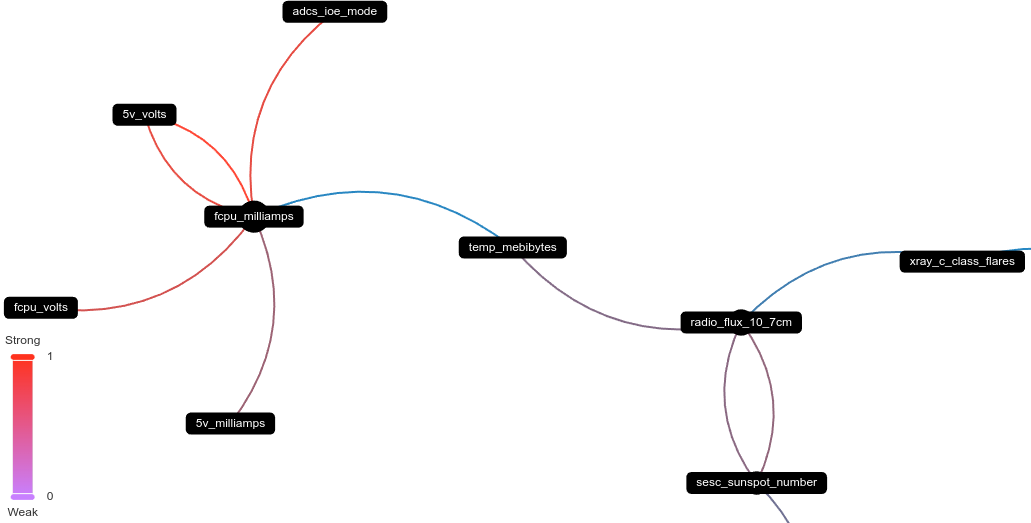
\includegraphics[width=0.95\textwidth]{sat/grifex_dgd.png}
	\caption{Граф кросс-корреляций для основных солнечных и геомагнитных индексов (GRIFEX)}
	\label{fig:grifex_dgd}
\end{figure}

\begin{figure}[H]
	\centering
	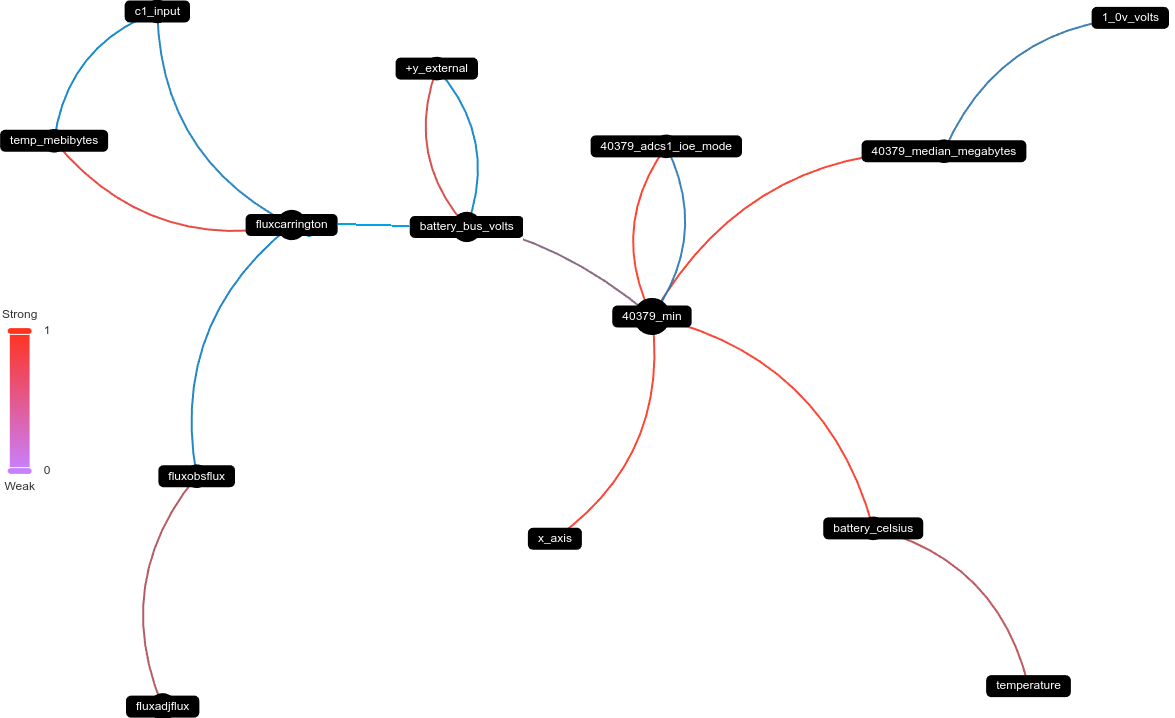
\includegraphics[width=0.95\textwidth]{sat/grifex_flux.png}
	\caption{Граф кросс-корреляций по потокам солнечного радиоизлучения (GRIFEX)}
	\label{fig:grifex_flux}
\end{figure}

\begin{figure}[H]
	\centering
	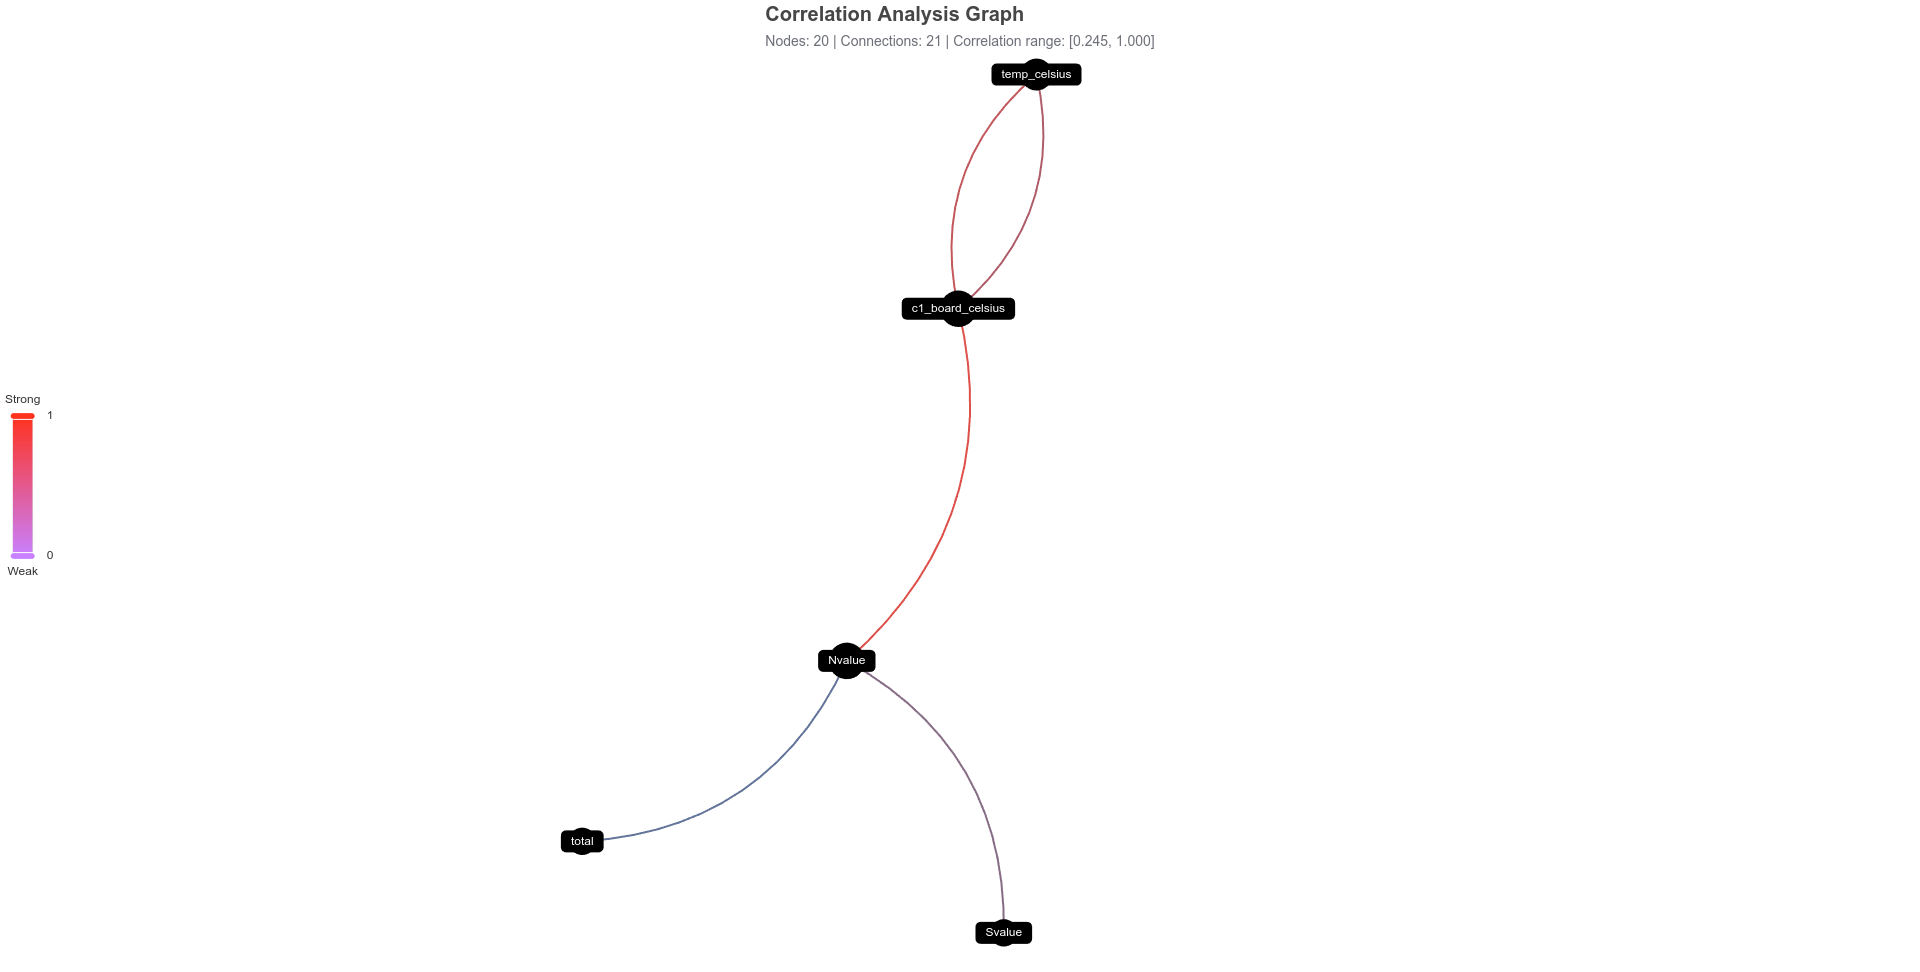
\includegraphics[width=0.95\textwidth]{sat/grifex_hemi.png}
	\caption{Граф кросс-корреляций по параметрам солнечных пятен по полушариям (GRIFEX)}
	\label{fig:grifex_hemi}
\end{figure}

\begin{figure}[H]
	\centering
	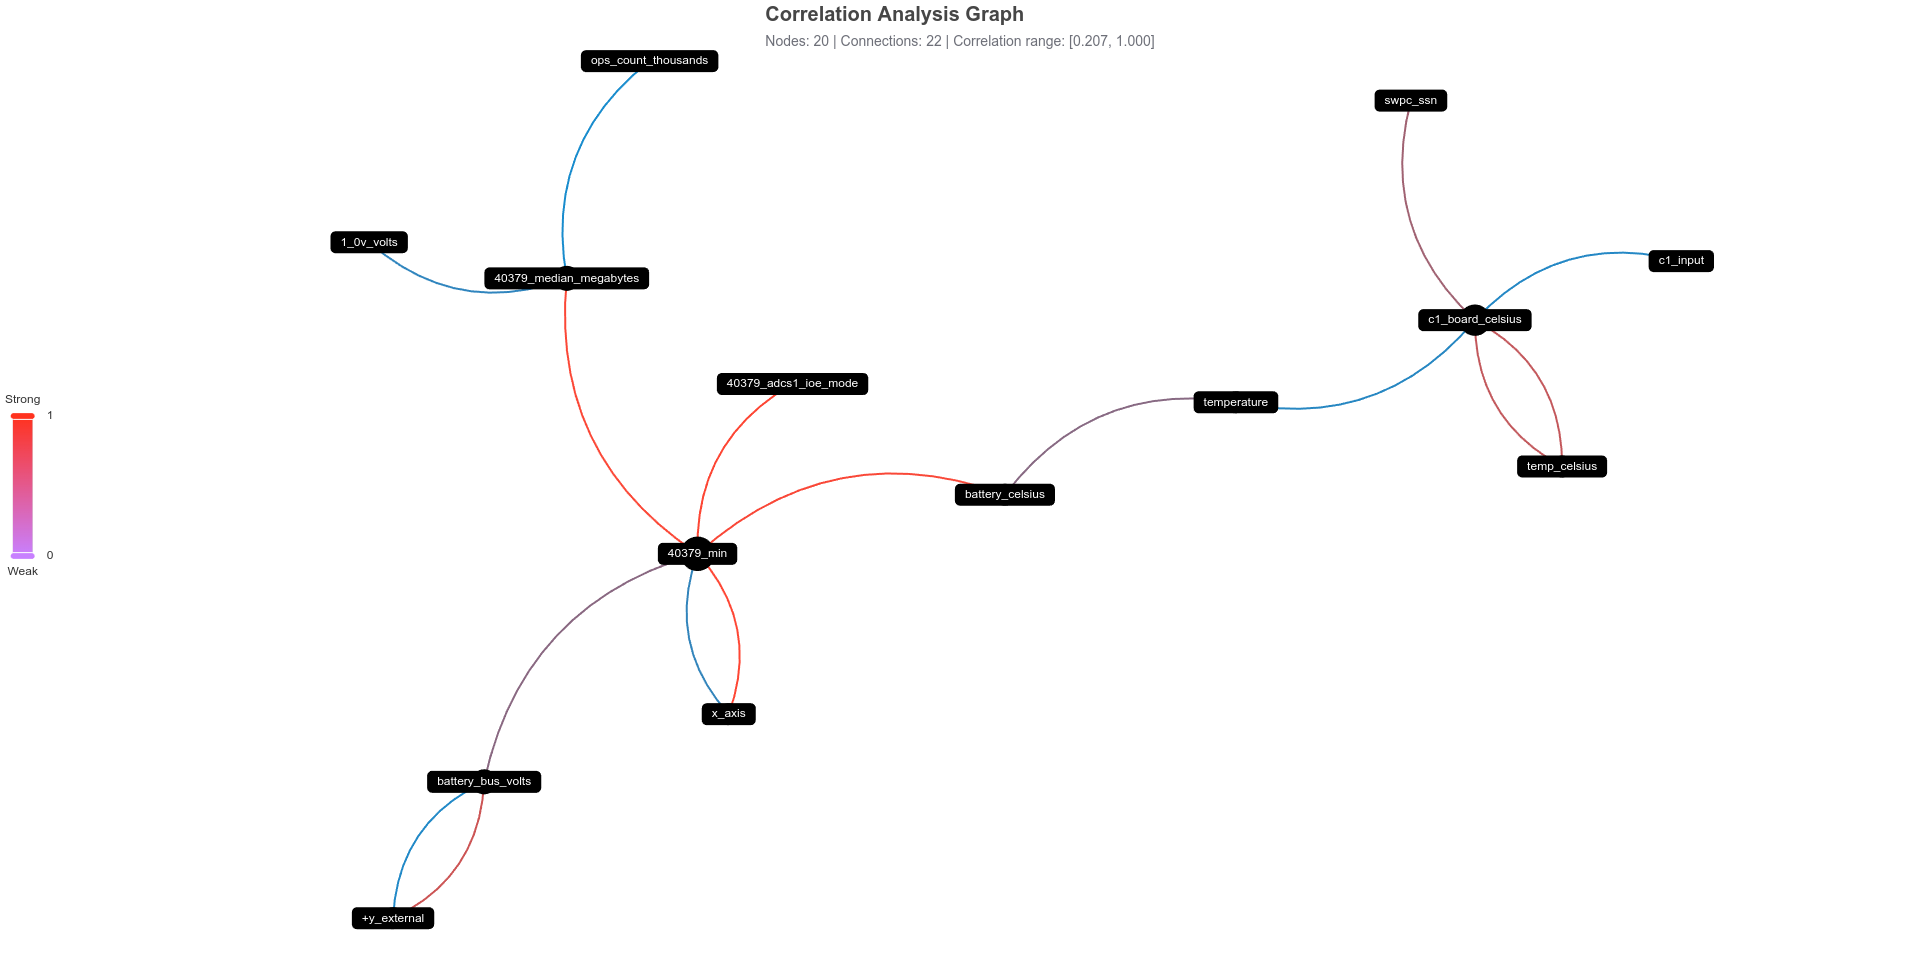
\includegraphics[width=0.95\textwidth]{sat/grifex_ssn.png}
	\caption{Граф кросс-корреляций по числу солнечных пятен (GRIFEX)}
	\label{fig:grifex_ssn}
\end{figure}

\subsection{Структурный анализ и физическая трактовка связей}

Анализируя структуру графов, можно отметить, что наибольшая плотность и сила
связей наблюдается между однородными параметрами солнечной активности, такими
как среднемесячное число солнечных пятен (\texttt{ssn}), сглаженное число пятен
(\texttt{smoothed\_ssn}), а также различные версии наблюдаемых и сглаженных
данных по числу пятен (\texttt{observed\_swpc\_ssn},
\texttt{smoothed\_swpc\_ssn}). Это объясняется тем, что все перечисленные
параметры отражают одну и ту же физическую сущность - магнитную активность на
поверхности Солнца, проявляющуюся в виде пятен, и различаются лишь методикой
усреднения и источником данных~\cite{sidc_manual}.

Потоки радиоизлучения (\texttt{f10.7}, \texttt{fluxobsflux},
\texttt{fluxadjflux}, \texttt{fluxursi}) также образуют тесно связанный кластер.
Данные параметры измеряются на длине волны 10,7 см и служат стандартом для
оценки уровня ультрафиолетового и рентгеновского излучения Солнца, оказывающего
непосредственное влияние на ионосферу и, как следствие, на работу радиосистем
спутника~\cite{f107_standard}. Сильные корреляции внутри этого кластера
подтверждают физическую однородность процессов генерации радиоизлучения на
Солнце.

В отличие от солнечных параметров, геомагнитные индексы (\texttt{Fredericksburg
	A}, \texttt{Fredericksburg K 0-3}, \texttt{K 3-6}, \texttt{K 6-9}) демонстрируют
более слабые и разреженные связи с солнечными показателями. Это связано с тем,
что геомагнитная активность - результат сложного взаимодействия солнечного ветра
и магнитосферы Земли, где задержки и нелинейные эффекты существенно ослабляют
прямую корреляцию~\cite{geomag_handbook}. Тем не менее, при анализе временных
рядов можно наблюдать, что периоды высокой солнечной активности (рост числа
пятен и потока F10.7) приводят к увеличению числа магнитных бурь и, как
следствие, к росту значений геомагнитных индексов.

Особый интерес представляет влияние солнечной активности на технические
параметры спутника GRIFEX. В отличие от большинства спутников класса CubeSat,
GRIFEX построен с применением инновационных архитектурных и технологических
решений, ориентированных на работу в условиях повышенного радиационного фона и
экстремальных температурных колебаний. Ключевой особенностью является использование гибридного матричного детектора (FPA, Focal Plane Array), представляющего собой двумерную матрицу детекторных элементов, в котором кремниевые SiPIN-диоды, произведённые Raytheon Vision Systems, интегрированы с современной БИС-схемой считывания (ROIC) с аналогово-цифровыми преобразователями в каждом пикселе~\cite{norton2012spaceborne, eoportal_grifex}.
Это решение обеспечивает
не только высокую помехоустойчивость, но и устойчивость к радиационным
воздействиям, что нетипично для стандартных CubeSat, традиционно использующих
коммерческие компоненты без специальной защиты.

Вся система управления и обработки данных построена на базе FPGA Xilinx
Virtex-5, что позволило реализовать отказоустойчивую архитектуру с минимизацией
числа точек отказа и резервированием ключевых функций~\cite{eoportal_grifex}.
Для GRIFEX были специально выбраны компоненты с повышенной радиационной
стойкостью: это касается как цифровых, так и аналоговых трактов. По данным MXL,
в конструкцию включены дополнительные экранирующие элементы, а также реализованы
алгоритмы коррекции ошибок памяти и мониторинга питания~\cite{mxl_grifex}.

Такой подход позволил существенно снизить количество сбоев и перезагрузок
аппаратуры даже в периоды экстремальных солнечных событий, что подтверждается
инженерными телеметрическими данными за весь период
эксплуатации~\cite{mxl_grifex}. В частности, при увеличении солнечной активности
наблюдается рост выработки энергии солнечными панелями, что приводит к повышению
токов и напряжений на бортовых шинах. Это, в свою очередь, способствует
поддержанию стабильной работы вычислительных блоков и уменьшению числа аварийных
перезапусков. Таким образом, положительное влияние солнечной активности
проявляется в увеличении энергетического ресурса спутника, при условии
эффективной защиты от радиационных воздействий.

На графах кросс-корреляций это выражается в виде сильных связей между
параметрами, характеризующими солнечную активность и электрические показатели
(ток, напряжение, температура панелей). В периоды низкой солнечной активности,
наоборот, возможно снижение выработки энергии, что увеличивает риск сбоев и
требует применения дополнительных мер энергосбережения.

Структурный анализ графов кросс-корреляций для спутника GRIFEX позволяет сделать
следующие выводы. Во-первых, высокая степень корреляции между однородными
солнечными параметрами подтверждает корректность и согласованность используемых
методик измерения. Во-вторых, относительно слабая связь между солнечными и
геомагнитными индексами обусловлена сложностью процессов передачи солнечного
воздействия через магнитосферу Земли. В-третьих, применение радиационно-стойких
материалов и архитектурных решений обеспечивает устойчивость аппаратуры к
солнечным вспышкам, а увеличение солнечной активности, как правило, приводит к
росту энергетических возможностей и снижению числа сбоев.

\section{ENSO}

\subsection{Структурные и технологические особенности}

ENSO (\textit{Expleo Nanosat for Solar-irradiance Observations}) - это
исследовательский 1U CubeSat, разработанный компанией Expleo совместно с
Университетским космическим центром Монпелье (CSUM) для задач мониторинга
солнечной активности и её влияния на ионосферу~\cite{expleo_enso_pdf,
	nanosats_enso, expleo_enso_launch}. Масса спутника составляет около 1 кг,
габариты - 10$\times$10$\times$10 см. ENSO оснащён развертываемой шестиметровой
антенной для передачи высокочастотного сигнала на наземные станции SANSA в
Антарктиде, а также камерой для вторичных задач сбора
данных~\cite{nanosats_enso, expleo_enso_launch}.

Конструкция спутника выполнена по классической схеме CubeSat: основной силовой
набор и панели изготовлены из алюминиевого сплава с анодированием для повышения
коррозионной стойкости и минимизации дегазации~\cite{expleo_enso_pdf,
	nanosats_enso}. Внутренние элементы электроники и крепежа используют стандартные
полимерные материалы, такие как полиимид (Kapton) для изоляции и защиты от
температурных перепадов, а также фторполимеры для кабельных
соединений~\cite{curbell_plastics}. Вся компонентная база построена на
коммерческих элементах (COTS), что характерно для современных малых спутников,
ориентированных на минимизацию стоимости и времени
разработки~\cite{expleo_enso_pdf, nanosats_enso}.

В отличие от специализированных радиационно-стойких платформ, в ENSO не
применяются rad-hard компоненты: устойчивость к космическим воздействиям
достигается за счёт оптимизации орбиты (низкая околоземная, минимизация времени
пребывания в радиационных поясах), базового экранирования алюминиевыми стенками
(толщина порядка 1–2 мм, что соответствует типичным рекомендациям NASA для
CubeSat~\cite{nasa_shielding}), а также программных методов коррекции ошибок
передачи и хранения данных~\cite{expleo_enso_pdf, nanosats_enso,
	nasa_shielding}. В ходе наземных испытаний ENSO прошёл тестирование на вибрации
и термовакуум, подтверждена работоспособность в диапазоне температур от –40°C до
+50°C в выключенном состоянии и от –20°C до +40°C в рабочем
режиме~\cite{expleo_enso_pdf}.

Таким образом, ENSO - типичный представитель NewSpace-подхода: лёгкая,
компактная платформа с минимальной массой, построенная на коммерческих
компонентах, с базовой защитой от радиации и температурных воздействий,
рассчитанная на ограниченный срок службы (до 4 лет) в условиях низкой
околоземной орбиты. Основная уязвимость - чувствительность к солнечным вспышкам
и радиационным событиям, что компенсируется резервированием каналов передачи и
программной устойчивостью~\cite{nasa_shielding, expleo_enso_pdf}.

\subsection{Структурный анализ}

В данном разделе рассматривается спутник ENSO, для которого построены графы
кросс-корреляций между инженерными и внешними параметрами
(рис.~\ref{fig:enso_sunspot}, \ref{fig:enso_ssn}, \ref{fig:enso_flux}). Для ENSO
проведён углублённый анализ структуры, особенностей используемых материалов и
архитектурных решений, а также рассмотрено влияние солнечной активности на
функционирование его систем.

\begin{figure}[H]
	\centering
	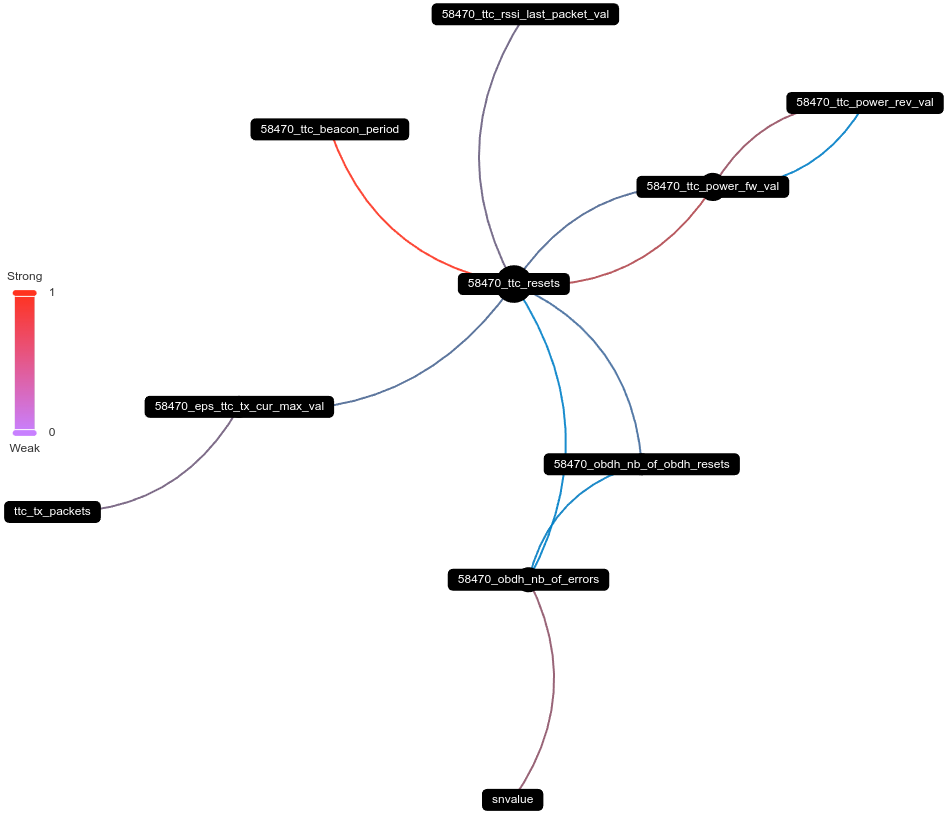
\includegraphics[width=0.95\textwidth]{sat/enso_sunspot.png}
	\caption{Граф кросс-корреляций по солнечным пятнам и инженерным параметрам (ENSO)}
	\label{fig:enso_sunspot}
\end{figure}

\begin{figure}[H]
	\centering
	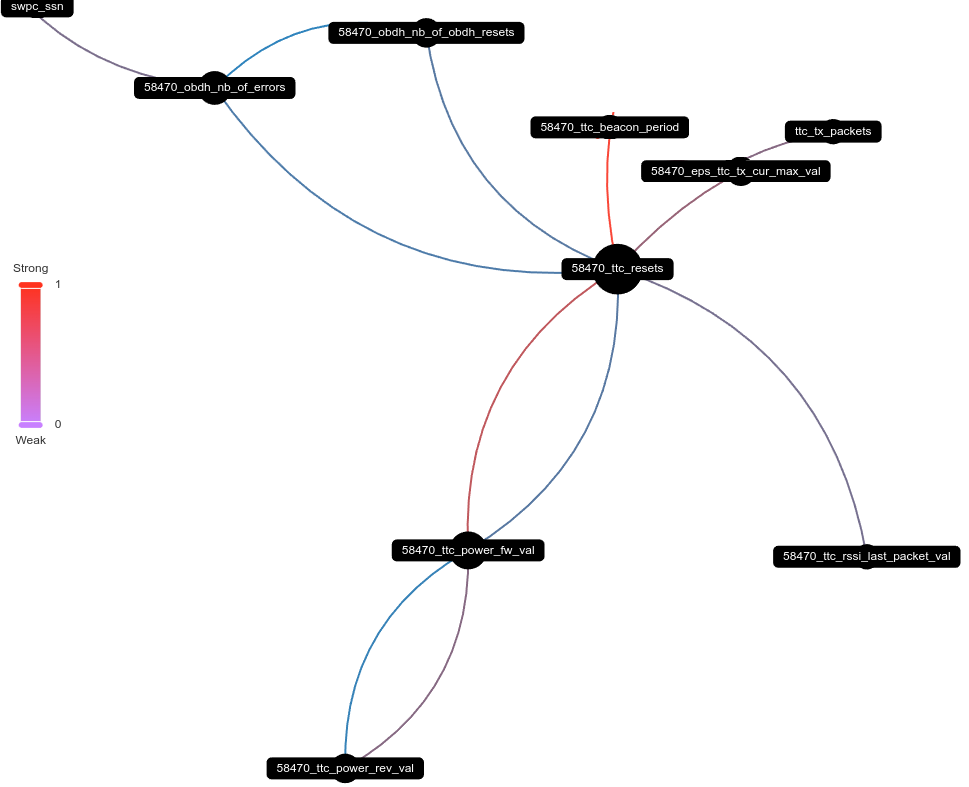
\includegraphics[width=0.95\textwidth]{sat/enso_ssn.png}
	\caption{Граф кросс-корреляций по числу солнечных пятен (ENSO)}
	\label{fig:enso_ssn}
\end{figure}

\begin{figure}[H]
	\centering
	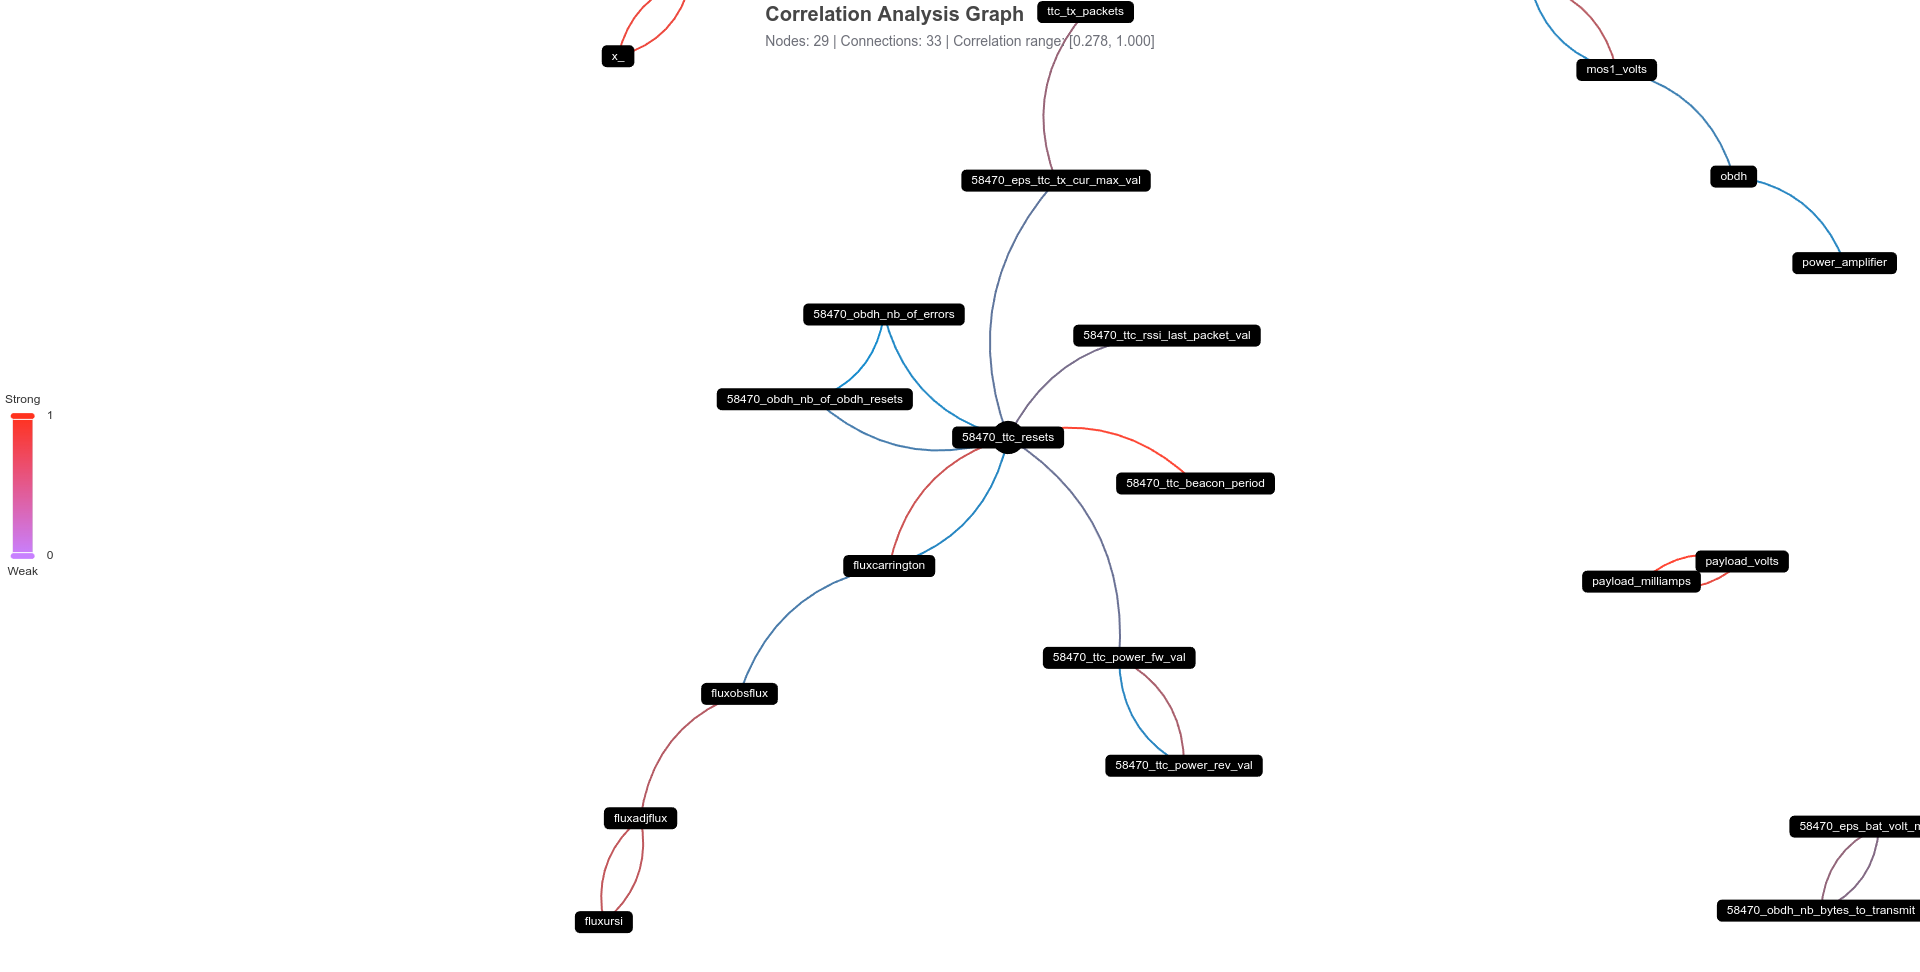
\includegraphics[width=0.95\textwidth]{sat/enso_flux.png}
	\caption{Граф кросс-корреляций по солнечному радиоизлучению (ENSO)}
	\label{fig:enso_flux}
\end{figure}

В центре большинства графов находится параметр \texttt{58470\_ttc\_resets} -
число перезапусков радиотехнического комплекса передачи данных. Этот параметр
тесно связан с ошибками и сбоями в подсистемах передачи и обработки информации
(\texttt{58470\_obdh\_nb\_of\_errors},
\texttt{58470\_obdh\_nb\_of\_obdh\_resets}), а также с энергетическими
характеристиками (\texttt{58470\_eps\_ttc\_bx\_cur\_max\_val},
\texttt{58470\_ttc\_power\_fw\_val}, \texttt{58470\_ttc\_power\_rev\_val}).

Анализ графа на рисунке~\ref{fig:enso_sunspot} показывает, что увеличение
количества ошибок и перезапусков в подсистемах (\texttt{obdh}, \texttt{ttc})
коррелирует с изменениями энергетических параметров. Связи между
\texttt{ttc\_resets} и \texttt{beacon\_period}, а также между
\texttt{ttc\_resets} и \texttt{ttc\_power\_fw/rev\_val} имеют различную силу:
наиболее сильные (красные рёбра) соответствуют случаям, когда сбои в питании или
перегрузки приводят к аварийным перезапускам радиотракта. Слабые (синие) и
средние (фиолетовые) связи фиксируют менее выраженные, но устойчивые зависимости
- например, рост тока передачи (\texttt{eps\_ttc\_bx\_cur\_max\_val}) при
увеличении числа пакетов (\texttt{ttc\_tx\_packets}), что отражает
закономерности работы CubeSat на низкой околоземной
орбите~\cite{expleo_enso_pdf}.

На графе~\ref{fig:enso_ssn} прослеживается связь между числом солнечных пятен
(\texttt{swpc\_ssn}) и инженерными параметрами. В периоды роста солнечной
активности наблюдается тенденция к снижению числа ошибок и перезапусков, что
связано с увеличением выработки энергии солнечными панелями и стабилизацией
работы энергетической подсистемы. Однако, при экстремальных событиях возможен
обратный эффект - рост числа сбоев из-за повышения радиационного
фона~\cite{nasa_shielding}.

Граф~\ref{fig:enso_flux} демонстрирует аналогичные закономерности для параметров
солнечного радиоизлучения (\texttt{fluxcarrington}, \texttt{fluxobsflux},
\texttt{fluxadjflux}, \texttt{fluxursi}). Сильные корреляции между током
нагрузки полезной нагрузки (\texttt{payload\_milliamps}) и напряжением
(\texttt{payload\_volts}) указывают на прямую зависимость между уровнем
солнечного излучения и энергетическими возможностями спутника. Связи между
параметрами питания и сбоями подтверждают, что энергетические провалы или
перегрузки приводят к увеличению числа перезапусков и ошибок в системах передачи
и обработки данных.

В периоды низкой солнечной активности возможно снижение напряжения и тока на
батареях (\texttt{eps\_bat\_volt\_avg\_val}, \texttt{battery\_voltage\_volts}),
что увеличивает риск сбоев и аварийных перезапусков. Это типично для малых
CubeSat, построенных на коммерческих компонентах без специализированной
радиационной защиты~\cite{expleo_enso_pdf, nanosats_enso}.


\section{Veronika}

\subsection{Структурные и технологические особенности}

Veronika - это 1U CubeSat, разработанный и произведённый словацкой компанией
Spacemanic при поддержке Deutsche Schule Bratislava, PLANETUM (Прага) и
Технического университета Кошице~\cite{spacemanic_veronika, nanosats_veronika,
	satnogs_veronika, kozmonautika_veronika}. Аппарат был выведен на
солнечно-синхронную орбиту высотой 550 км 11 ноября 2023 года ракетой Falcon 9
(миссия Transporter-9). Масса спутника составляет 1010 г, размеры - стандартный
1U форм-фактор.

Конструкция Veronika выполнена с использованием проверенных компонентов с
богатой летной историей, разработанных и интегрированных компанией
Spacemanic~\cite{spacemanic_veronika, nanosats_veronika}. Корпус изготовлен из
анодированного алюминиевого сплава, что обеспечивает необходимую механическую
прочность и минимальный уровень дегазации. Для электроизоляции и защиты от
температурных перепадов применяются полиимидные материалы (например, Kapton), а
для крепежа и кабельных соединений - стандартные полимерные материалы,
используемые в индустрии малых спутников~\cite{spacemanic_veronika,
	kozmonautika_veronika}.

На борту установлены две камеры (uCAM и iCAM) для съёмки Земли, каждая из
которых отличается компактностью, малой массой и низким энергопотреблением. uCAM
- это малогабаритная камера с разрешением до 640 на 480, CMOS-сенсором и углом
обзора 116°, а iCAM - более лёгкая камера с VGA-разрешением и углом обзора
60°~\cite{kozmonautika_veronika}.

Энергетическая подсистема включает солнечные панели и аккумуляторную батарею,
обеспечивающие питание всех систем CubeSat. Радиокомплекс поддерживает работу в
любительских диапазонах UHF (436.680 МГц) и VHF (145.925 МГц), реализованы
протоколы AX.25, GFSK и CW для передачи телеметрии и пользовательских
сообщений~\cite{spacemanic_veronika, nanosats_veronika, kozmonautika_veronika}.
Важной особенностью является наличие экспериментальной системы ориентации (ADCS)
с электромагнитными приводами и приёмником GNSS, что позволяет спутнику
стабилизироваться и определять своё положение в
пространстве~\cite{spacemanic_veronika, nanosats_veronika}.

Вся компонентная база - коммерческая (COTS), без применения специализированных
радиационно-стойких решений, что типично для современных образовательных и
технологических CubeSat~\cite{spacemanic_veronika, nanosats_veronika, nasa_soa}.
Перед запуском Veronika прошла полный цикл испытаний на вибрацию, термовакуум и
электромагнитную совместимость, что подтверждено инженерными отчётами
компании~\cite{spacemanic_veronika, kozmonautika_veronika}.

\subsection{Анализ графов кросс-корреляций}

На рисунках~\ref{fig:veronika_sunspot}--\ref{fig:veronika_flux} представлены
графы кросс-корреляций между инженерными и внешними параметрами спутника
Veronika.

\begin{figure}[H]
	\centering
	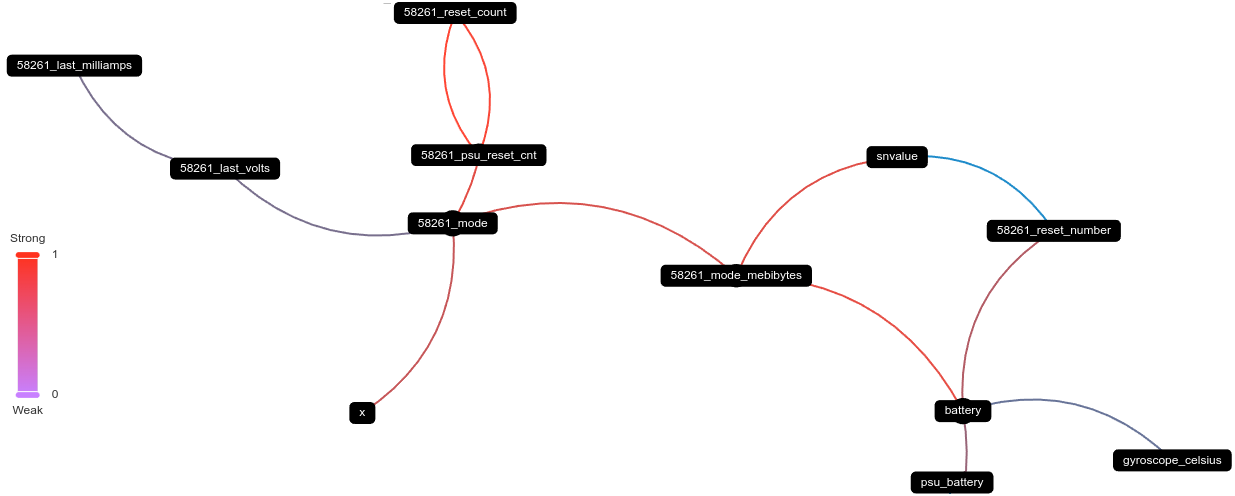
\includegraphics[width=0.95\textwidth]{sat/veronika_sunspot.png}
	\caption{Граф кросс-корреляций по инженерным параметрам и солнечным пятнам (Veronika)}
	\label{fig:veronika_sunspot}
\end{figure}

\begin{figure}[H]
	\centering
	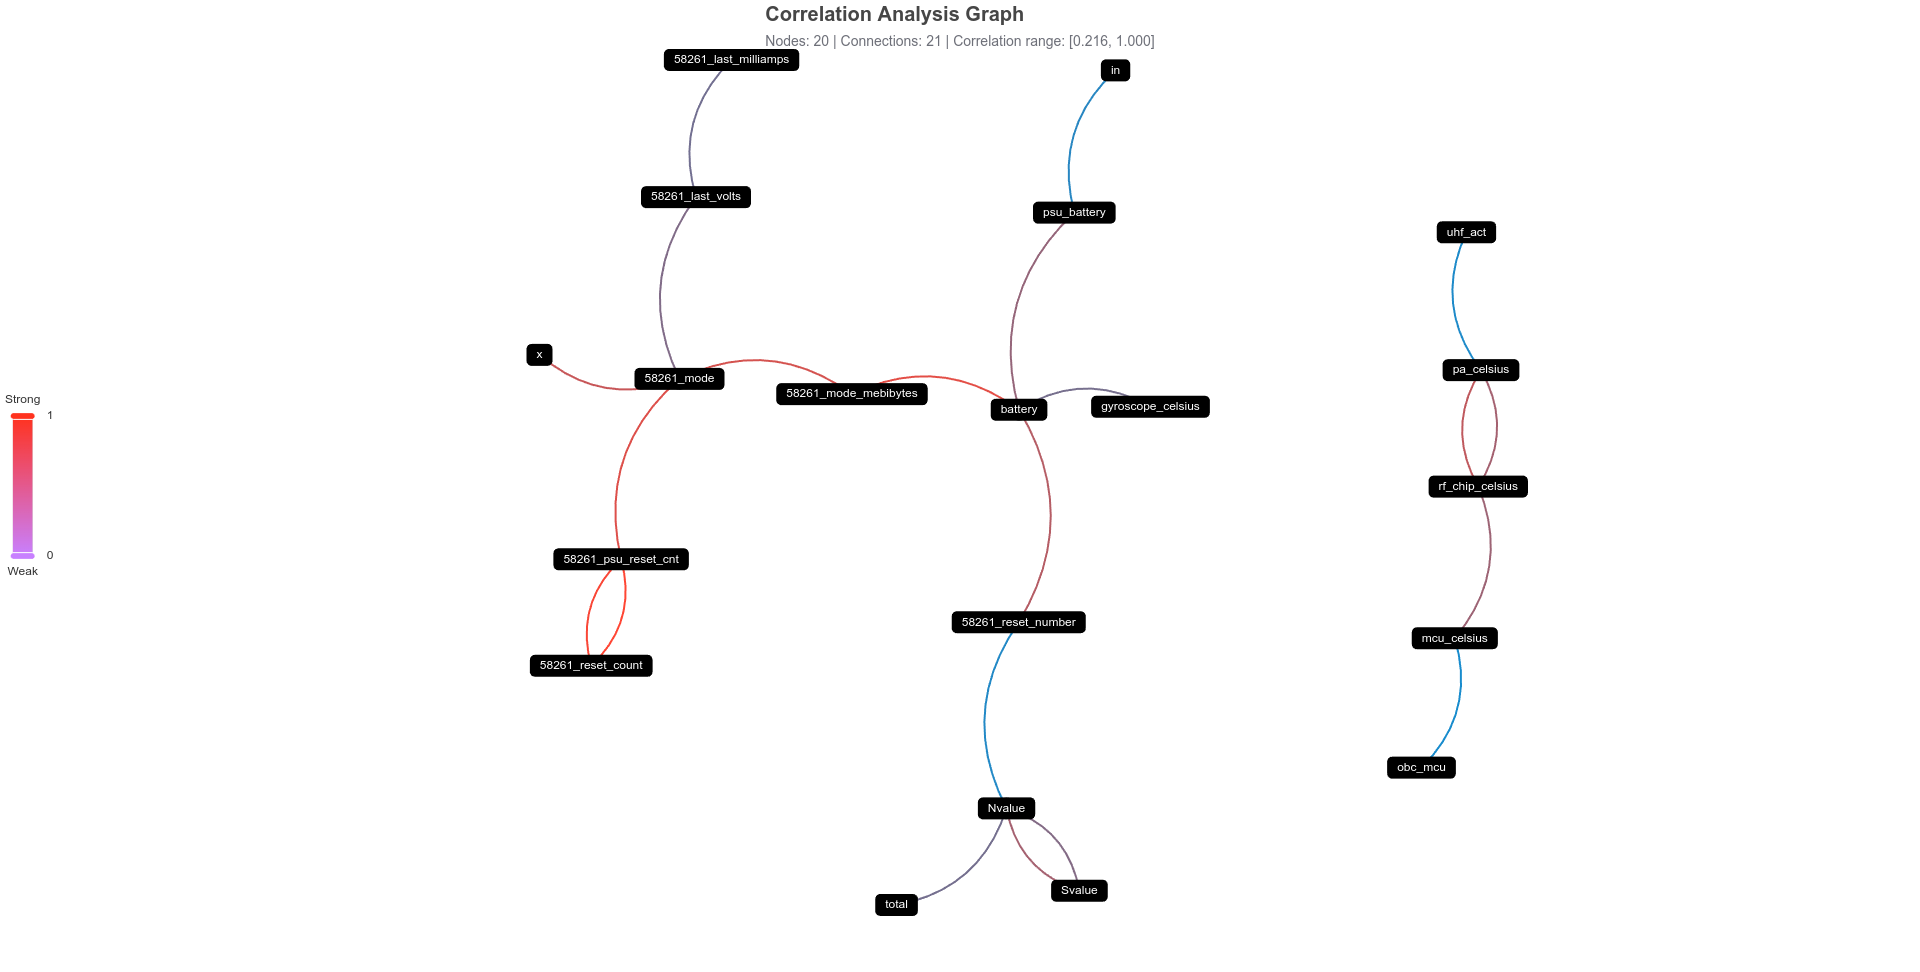
\includegraphics[width=0.95\textwidth]{sat/veronika_hemi.png}
	\caption{Граф кросс-корреляций по гемиcферическим числам солнечных пятен (Veronika)}
	\label{fig:veronika_hemi}
\end{figure}

\begin{figure}[H]
	\centering
	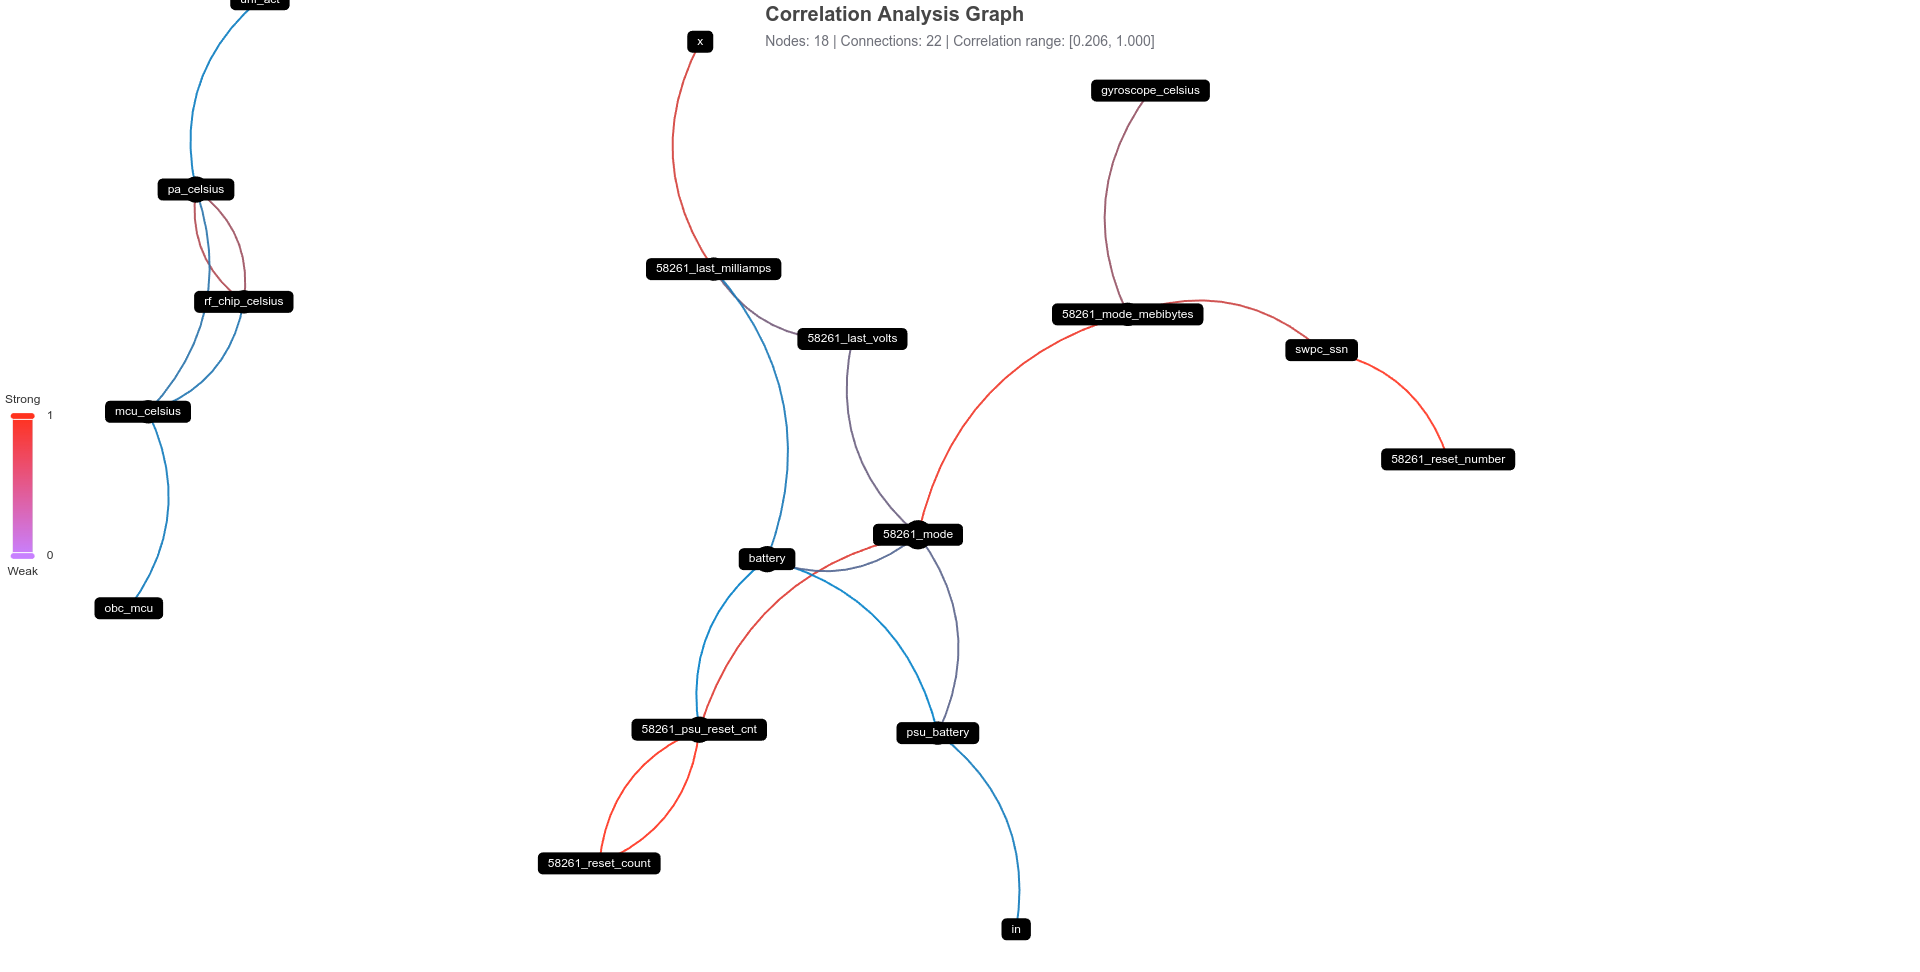
\includegraphics[width=0.95\textwidth]{sat/veronika_ssn.png}
	\caption{Граф кросс-корреляций по среднемесячному числу солнечных пятен (Veronika)}
	\label{fig:veronika_ssn}
\end{figure}

\begin{figure}[H]
	\centering
	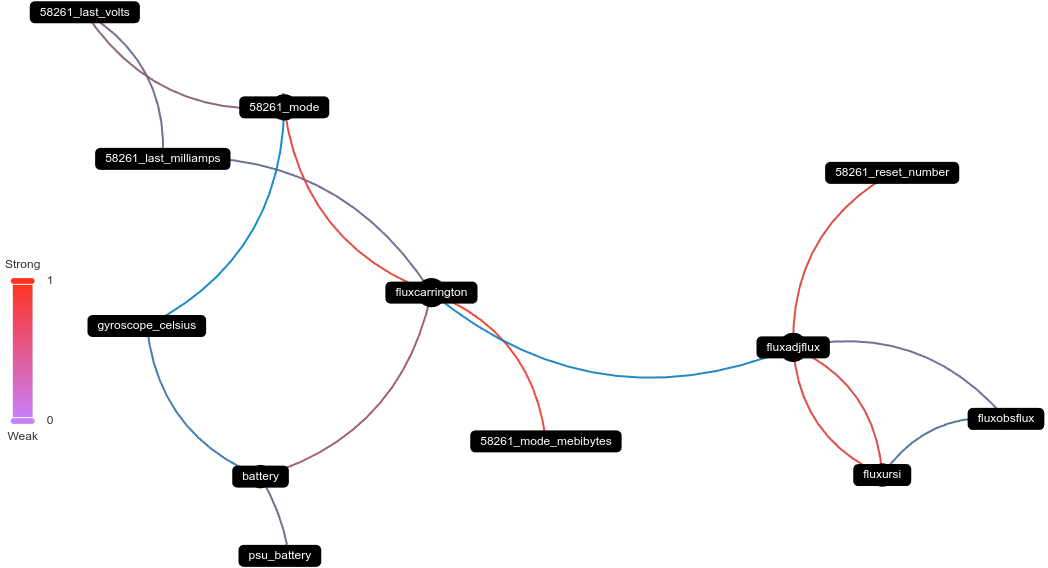
\includegraphics[width=0.95\textwidth]{sat/veronika_flux.png}
	\caption{Граф кросс-корреляций по солнечному радиоизлучению (Veronika)}
	\label{fig:veronika_flux}
\end{figure}


В центре представленных графов кросс-корреляций для спутника Veronika
(рис.~\ref{fig:veronika_sunspot}--\ref{fig:veronika_flux}) находятся параметры,
связанные не только с энергетикой, но и с логикой функционирования, сбоями и
тепловыми режимами ключевых подсистем. Наиболее сильные корреляции (красные
рёбра) фиксируются между счетчиками перезапусков (\texttt{58261\_reset\_count},
\texttt{58261\_psu\_reset\_cnt}, \texttt{58261\_reset\_number}) и рабочими
режимами (\texttt{58261\_mode}, \texttt{58261\_mode\_mebbytes}), что указывает
на прямую зависимость надёжности работы от переходов между режимами и состояния
управляющей электроники. Это типично для малых спутников с ограниченными
ресурсами: сбои часто инициируются не только энергетическими провалами, но и
логическими ошибками, накоплением ошибок памяти или перегревом
микроконтроллеров~\cite{spacemanic_veronika, nanosats_veronika}.

Графы демонстрируют, что влияние солнечной активности на Veronika не является
однозначно положительным. С одной стороны, рост солнечной активности (параметры
\texttt{swpc\_ssn}, \texttt{fluxcarrington}, \texttt{fluxobsflux},
\texttt{fluxadjflux}, \texttt{fluxursi}) приводит к увеличению выработки энергии
солнечными панелями, что проявляется в корреляциях между током нагрузки
(\texttt{58261\_last\_milliamps}), напряжением (\texttt{58261\_last\_volts},
\texttt{battery}, \texttt{psu\_battery}) и снижением числа аварийных
перезапусков~\cite{spacemanic_veronika, nanosats_veronika}. Однако при
экстремальных вспышках и магнитных бурях наблюдается усиление негативных
эффектов: возрастает количество сбоев, увеличивается число аппаратных
перезапусков, фиксируются скачки температур в чувствительных узлах (кластер
температурных параметров: \texttt{mcu\_celsius}, \texttt{rf\_chip\_celsius},
\texttt{pa\_celsius}, \texttt{uhf\_act}, \texttt{obc\_mcu})~\cite{nasa_soa,
	stehlikova_veronika}.

Особо стоит отметить, что корреляции между температурными параметрами и сбоями
не всегда линейны: перегрев радиотракта или управляющего микроконтроллера
(\texttt{mcu\_celsius}, \texttt{rf\_chip\_celsius}) может быть как следствием
интенсивной работы в условиях высокой солнечной активности, так и результатом
внутренних сбоев, вызванных, например, ошибками в логике управления питанием. В
ряде случаев наблюдается каскадный эффект: рост солнечной активности
$\rightarrow$ увеличение выработки энергии $\rightarrow$ рост нагрузки на
радиотракт $\rightarrow$ рост температуры $\rightarrow$ увеличение вероятности
аппаратных сбоев и перезапусков~\cite{stehlikova_veronika, spacemanic_veronika}.

Связи между параметрами \texttt{battery}, \texttt{psu\_battery},
\texttt{last\_milliamps}, \texttt{last\_volts} и внешними индексами солнечной
активности подтверждают, что энергетическая стабильность - лишь один из факторов
надёжности. При недостатке солнечной энергии (низкая активность или затенение
орбиты) риск сбоев увеличивается из-за разрядки батарей, однако при избыточной
активности возможны перегревы и повреждения электроники, особенно в отсутствие
специализированной радиационной и тепловой защиты, как у
Veronika~\cite{spacemanic_veronika, stehlikova_veronika}.


\section{LASARsat}

\subsection{Структурные и технологические особенности}

LASARsat (Laser-Assisted Satellite Reentry satellite) представляет собой чешский
научный микроспутник формата 1U CubeSat, разработанный чешской школьной командой
LASAR при поддержке компаний Spacemanic, HiLASE, VZLU, SkyFox Labs и
Planetum~\cite{lasar_info, spacemanic_lasarsat, wiki_lasarsat}. Аппарат был
запущен на низкую околоземную орбиту 21 декабря 2024 года ракетой-носителем
Falcon 9 в рамках миссии Bandwagon-2. Масса спутника составляет 1085 г, размеры
- $10 \times 10 \times 11.3$ см, что соответствует расширенному формату
1U~\cite{wiki_lasarsat, spacemanic_lasarsat, satnogs_lasarsat}.

Конструкция LASARsat выполнена с использованием проверенных компонентов с
богатым лётным наследием, разработанных и интегрированных компанией
Spacemanic~\cite{spacemanic_lasarsat}. Корпус изготовлен из анодированного
алюминия с дополнительными элементами из композитных материалов, что
обеспечивает необходимую механическую прочность при минимальной массе.
Отличительной особенностью LASARsat является наличие специализированного
функционального оборудования для лазерных экспериментов, включая параболическое
зеркало для фокусировки лазерного излучения на абляционном
материале~\cite{satnogs_lasarsat, lasar_info}.

Спутник оснащён семью научными приборами~\cite{wiki_lasarsat, lasar_info}:
\begin{itemize}[wide]
	\item Фотодиоды (Solar Panel Photodiodes) - для измерения потерь энергии лазера при прохождении через атмосферу Земли;
	\item Светодиоды (LED) - для улучшения точности отслеживания спутника с Земли;
	\item Ретрорефлекторы - для отражения лазерного луча обратно на Землю и его дальнейшего изучения;
	\item Зонд Ленгмюра - для измерения изменений ионизации при воздействии лазера;
	\item Earthcam - камера для съёмки поверхности Земли и тестирования воздействия лазерного луча на оптические сенсоры;
	\item Два дозиметра - для измерения радиационного фона, предоставленные Чешским аэрокосмическим исследовательским центром и SkyFox Labs.
\end{itemize}

Энергетическая подсистема включает солнечные панели с фотодиодами (\texttt{zn} в
телеметрии) и аккумуляторную батарею, обеспечивающие питание всех систем
CubeSat. Радиокомплекс работает в любительском диапазоне UHF (436.925 МГц),
использует модуляции GFSK и CW для передачи телеметрии и пользовательских
сообщений~\cite{satnogs_lasarsat, spacemanic_lasarsat}. Система определения
ориентации и стабилизации интегрирована с GNSS-приёмником, качество работы
которого отражается в телеметрическом параметре \texttt{\_mode} (GNSS DOP -
снижение точности)~\cite{spacemanic_lasarsat, satnogs_lasarsat}.

\subsection{Анализ графов кросс-корреляций}

Представленные графы кросс-корреляций
(рис.~\ref{fig:lasarsat_sunspot},
\ref{fig:lasarsat_ssn},
\ref{fig:lasarsat_dgd},
\ref{fig:lasarsat_flux})
демонстрируют сложную структуру взаимосвязей между параметрами солнечной
активности и техническими показателями спутника LASARsat. Каждый узел графа
соответствует конкретному параметру, рёбра отражают наличие статистически
значимой корреляции, а их цвет кодирует силу связи: от синего (слабая) до
красного (сильная).

\begin{figure}[H]
	\centering
	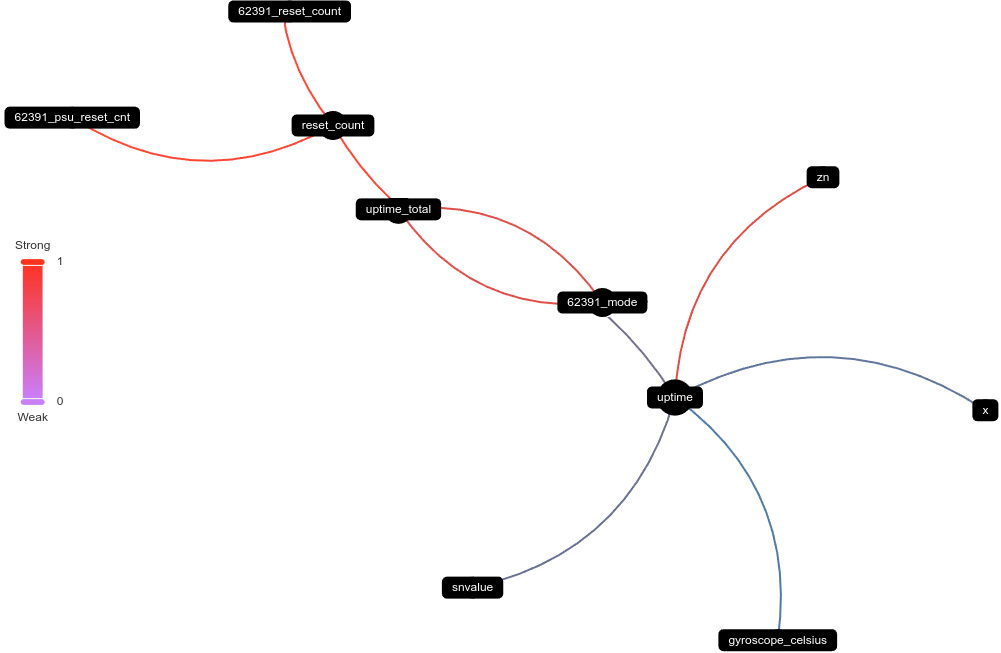
\includegraphics[width=0.95\textwidth]{sat/lasarsat_sunspot.png}
	\caption{Граф кросс-корреляций по солнечным пятнам и инженерным параметрам (LASARsat)}
	\label{fig:lasarsat_sunspot}
\end{figure}

\begin{figure}[H]
	\centering
	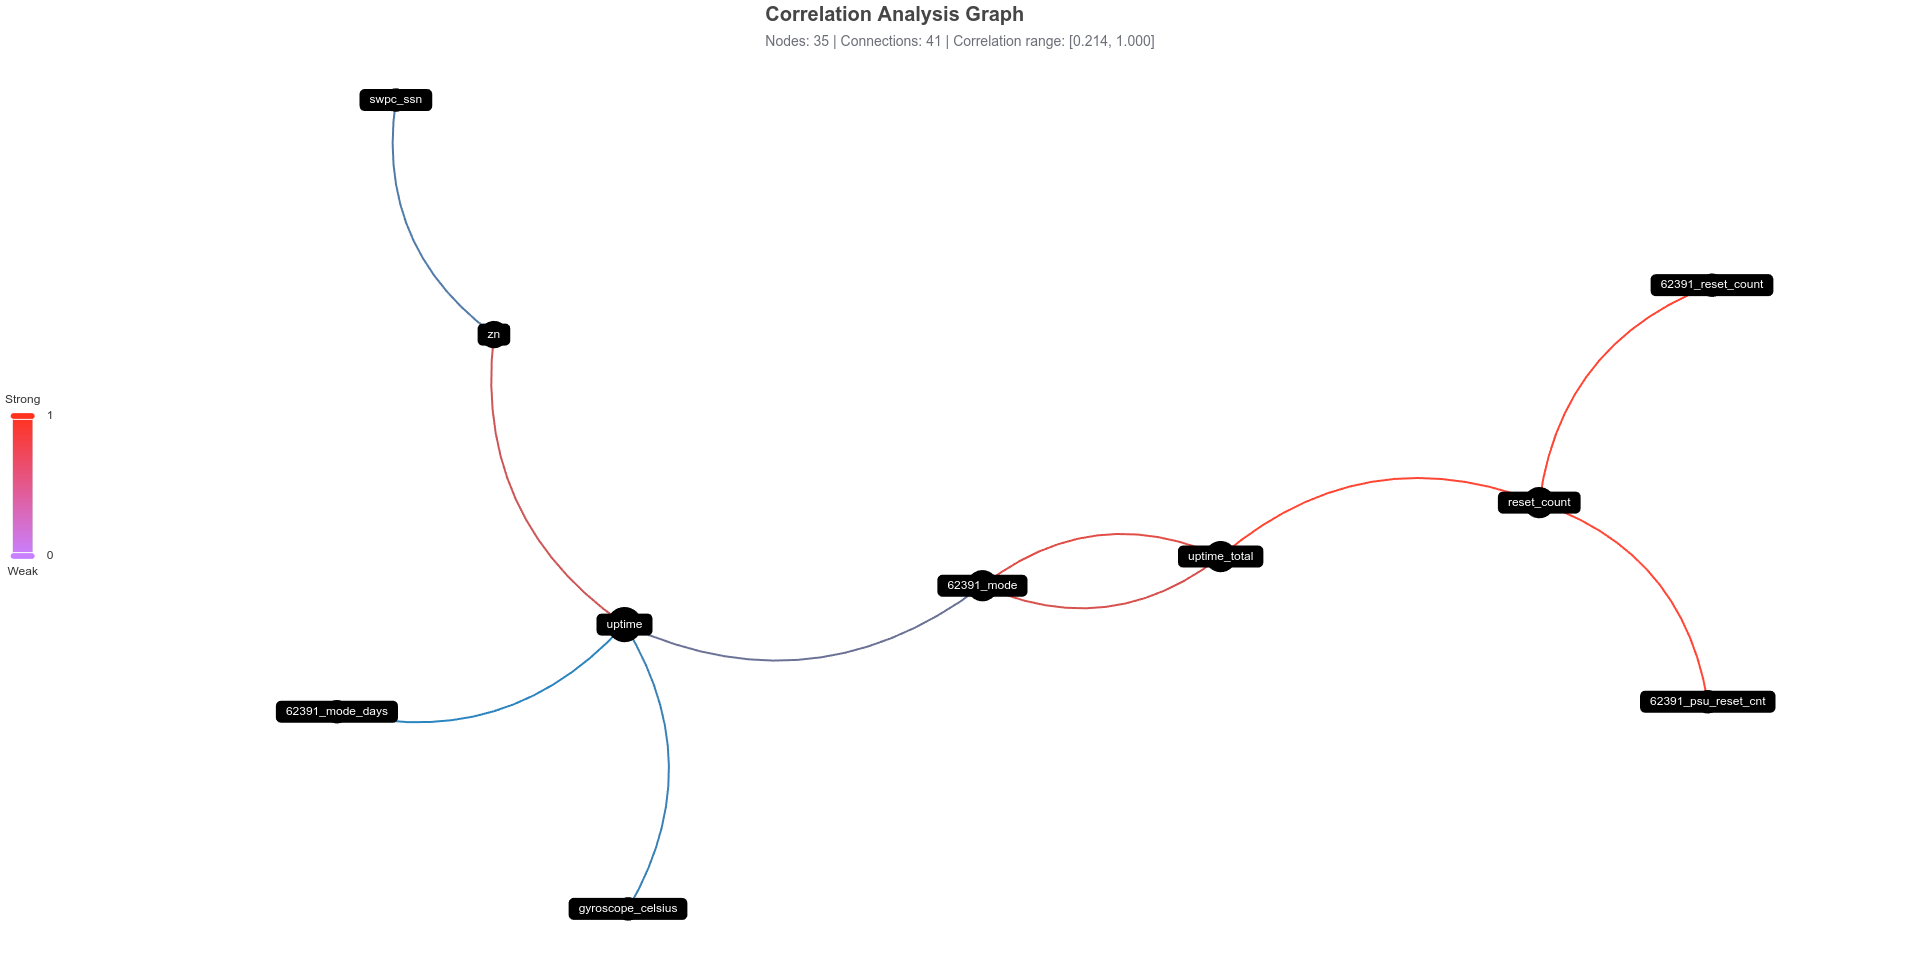
\includegraphics[width=0.95\textwidth]{sat/lasarsat_ssn.png}
	\caption{Граф кросс-корреляций по числу солнечных пятен (LASARsat)}
	\label{fig:lasarsat_ssn}
\end{figure}

\begin{figure}[H]
	\centering
	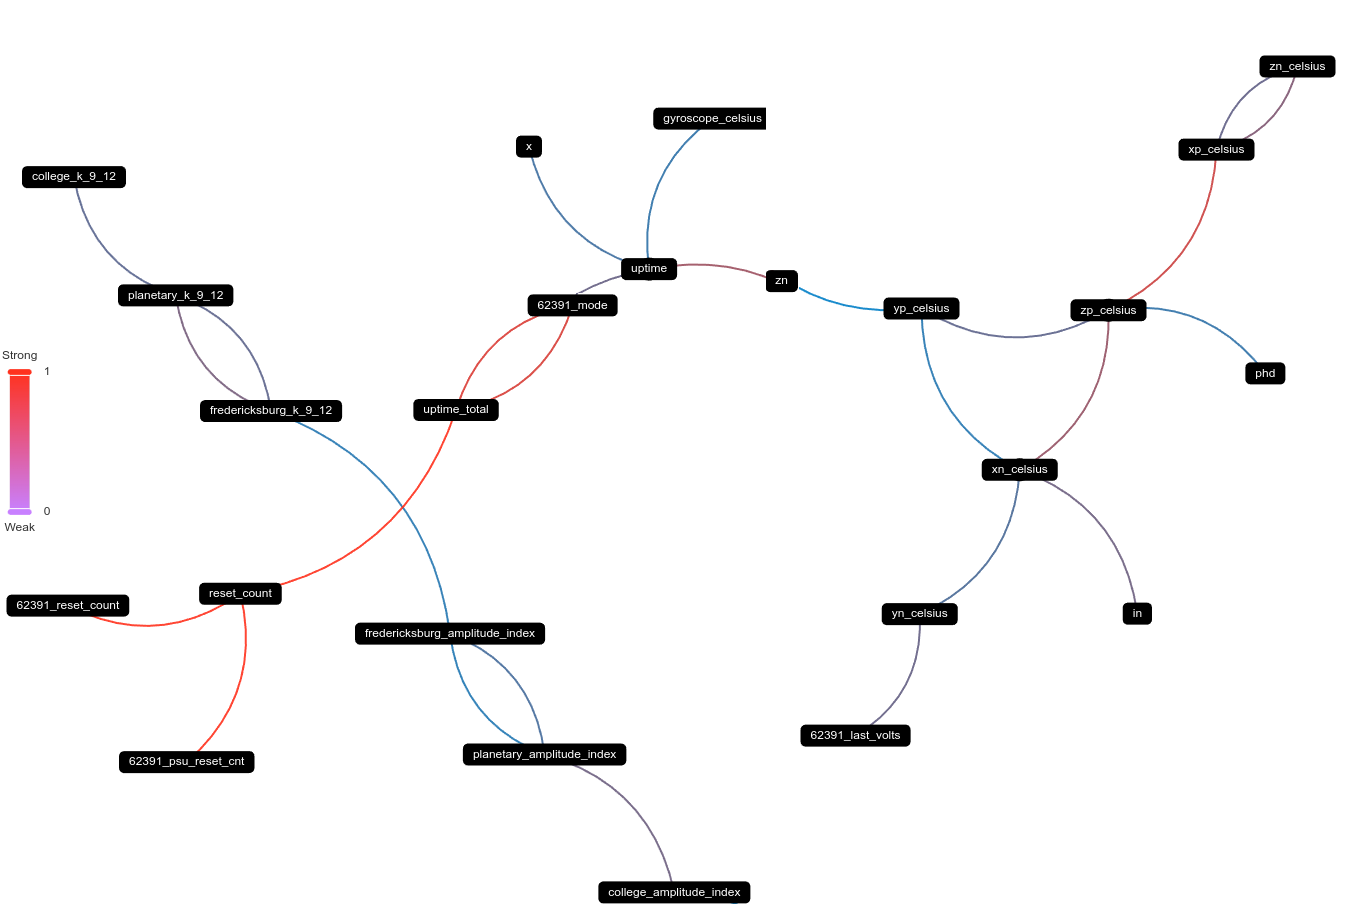
\includegraphics[width=0.95\textwidth]{sat/lasarsat_dgd.png}
	\caption{Граф кросс-корреляций по основным солнечным и геомагнитным индексам (LASARsat)}
	\label{fig:lasarsat_dgd}
\end{figure}

\begin{figure}[H]
	\centering
	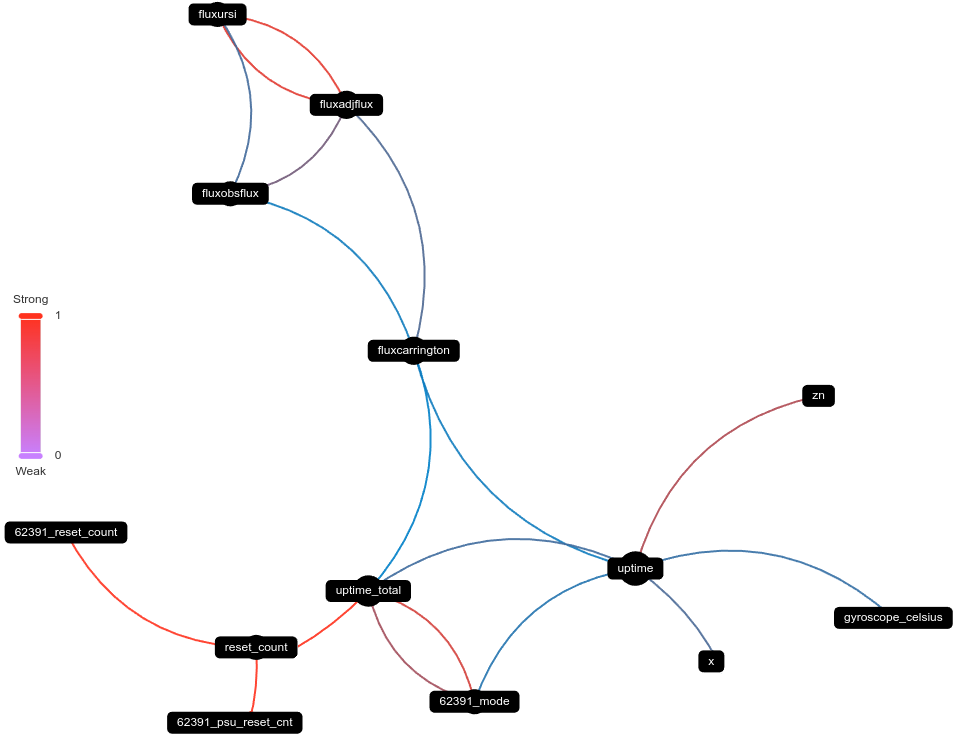
\includegraphics[width=0.95\textwidth]{sat/lasarsat_flux.png}
	\caption{Граф кросс-корреляций по солнечному радиоизлучению (LASARsat)}
	\label{fig:lasarsat_flux}
\end{figure}

В центре большинства графов находятся параметры счётчиков перезапусков
(\texttt{62391\_reset\_count}, \texttt{reset\_count},
\texttt{62391\_psu\_reset\_cnt}), времени активности (\texttt{uptime},
\texttt{uptime\_total}) и режимов работы (\texttt{62391\_mode}). Наиболее
сильные корреляции (красные рёбра) наблюдаются между счётчиками перезапусков и
режимами работы, что указывает на критическую зависимость стабильности
функционирования от внутренних состояний бортовых систем. Эта картина типична
для экспериментальных CubeSat, выполняющих сложные научные задачи при жёстких
ресурсных ограничениях~\cite{spacemanic_lasarsat, wiki_lasarsat}.

На графе рис.~\ref{fig:lasarsat_sunspot}
особого
внимания заслуживает слабое ребро (синего цвета) между показателем солнечной
активности \texttt{swpc\_ssn} и параметром \texttt{zn}. Это подтверждает влияние
солнечной активности на показания фотодиодов солнечных панелей, но слабая
корреляция указывает на наличие других существенных факторов, определяющих эти
показания - ориентация спутника, затенение, температурный
режим~\cite{lasar_info, spacemanic_lasarsat}. Одновременно заметна взаимосвязь
между \texttt{zn} и \texttt{uptime}, что свидетельствует о влиянии
энергетического состояния на продолжительность непрерывной работы аппаратуры.

Особый интерес представляют корреляции между \texttt{gyroscope\_celsius} и
параметрами режимов работы. Гироскопический датчик, будучи частью системы
определения ориентации, напрямую связан с динамическим состоянием спутника.
Повышение его температуры может быть следствием как интенсивной работы, так и
воздействия внешних факторов (солнечное излучение, геомагнитные возмущения).
Серия средних по силе связей (фиолетовые рёбра) между температурными параметрами
(\texttt{gyroscope\_celsius}, \texttt{yp\_celsius}, \texttt{yn\_celsius},
\texttt{zp\_celsius}, \texttt{zn\_celsius}) указывает на сложную тепловую
динамику внутри компактного корпуса CubeSat~\cite{wiki_lasarsat,
	spacemanic_lasarsat}.

На графе рис.~\ref{fig:lasarsat_flux}
прослеживается
связь между параметрами солнечного радиоизлучения (\texttt{fluxursi},
\texttt{fluxobsflux}, \texttt{fluxadjflux}, \texttt{fluxcarrington}) и
внутренними характеристиками спутника. В отличие от простой зависимости "больше
солнца - больше энергии", наблюдается комплексное влияние: увеличение потока
радиоизлучения приводит к росту температуры компонентов, что может как
стабилизировать работу отдельных подсистем, так и провоцировать сбои при
превышении критических значений~\cite{lasar_info, satnogs_lasarsat}.

Анализ графа рис.~\ref{fig:lasarsat_dgd}
выявляет
связи между геомагнитными индексами (\texttt{fredericksburg\_k\_9\_12},
\texttt{fredericksburg\_amplitude\_index}) и параметрами \texttt{reset\_count},
что подтверждает уязвимость электроники спутника к геомагнитным возмущениям. При
усилении магнитных бурь возрастает вероятность сбоев, особенно в
микроконтроллерах и памяти, что приводит к аварийным перезапускам и нарушениям в
работе научной аппаратуры~\cite{wiki_lasarsat, satnogs_lasarsat}.

Сложная взаимосвязь между \texttt{uptime}, \texttt{uptime\_total},
\texttt{reset\_count} и солнечными параметрами демонстрирует неоднозначность
влияния космической погоды на работу LASARsat. В определённом диапазоне значений
солнечной активности наблюдается положительный эффект (стабилизация
энергоснабжения, уменьшение числа перезапусков), однако при экстремальных
значениях или быстрых изменениях возникают каскадные эффекты: перегрев
$\rightarrow$ ошибки в работе сенсоров $\rightarrow$ нарушения в системе
ориентации $\rightarrow$ снижение энергетической эффективности $\rightarrow$
перезапуски~\cite{spacemanic_lasarsat, satnogs_lasarsat}.


\section{INSPIRESat-1}

\subsection{Структурные и технологические особенности}

INSPIRESat-1 (International Satellite Program in Research and Education
Satellite-1) представляет собой 9U CubeSat весом 8.6 кг и размерами $290 \times 200 \times
	160$ мм, разработанный международным консорциумом университетов, включая
Лабораторию атмосферной и космической физики Университета Колорадо (UC/LASP),
Индийский институт космической науки и технологий (IIST) и Национальный
центральный университет Тайваня (NCU)~\cite{eoportal_inspiresat,
	nanosats_inspiresat}. Спутник был запущен 14 февраля 2022 года ракетой-носителем
PSLV (C52) на солнечно-синхронную орбиту.

Научные цели миссии включают улучшение понимания динамики ионосферы через
наблюдения за температурой, составом, плотностью и скоростью ионов, а также
изучение процессов нагрева солнечной короны~\cite{eoportal_inspiresat,
	satnogs_inspiresat}. Для этого на борту установлены два основных научных
прибора:

\begin{itemize}
	\item Compact Ionosphere Probe (CIP) - комплексный плазменный датчик,
	      разработанный NCU для изучения ионосферы;
	\item Dual Aperture X-ray Solar Spectrometer (DAXSS) - спектрометр мягкого
	      рентгеновского излучения, разработанный LASP для измерения солнечного
	      спектра.
\end{itemize}

В отличие от многих коммерческих CubeSat, большинство компонентов INSPIRESat-1
разработаны непосредственно участниками консорциума. Командный блок и система
обработки данных (C\&DH), а также система электропитания (EPS) созданы IIST, в
то время как структурные и тепловые компоненты разработаны
LASP~\cite{core_inspiresat}. Система определения и контроля ориентации (ADCS) и
коммуникационные системы основаны на уже доступных решениях LASP и NCU.

Коммуникационная подсистема включает УВЧ-трансивер TRX-U от SpaceQuest с
возможностью передачи и приёма на скоростях от 2.4 кбит/с до 19.2 кбит/с, а
также S-диапазонный передатчик STX от Clyde Space~\cite{core_inspiresat}. Для
УВЧ-диапазона используется ленточная антенна, а для обеспечения высокоскоростной
связи в S-диапазоне - патч-антенна CPUT SANT с левой круговой поляризацией и
коэффициентом усиления до 8 дБи~\cite{core_inspiresat}.

Отличительной особенностью миссии является активное участие студентов в
проектировании, тестировании и эксплуатации спутника, что соответствует
образовательным целям программы INSPIRE~\cite{nanosats_inspiresat,
	satnogs_inspiresat}. Основная команда включает более 20 студентов и
преподавателей из IIST (Индия), Университета Колорадо Боулдер и NCU (Тайвань).

\subsection{Анализ графов кросс-корреляций}

Представленные графы кросс-корреляций
(рис.~\ref{fig:inspiresat_sunspot},
\ref{fig:inspiresat_hemi},
\ref{fig:inspiresat_flux},
\ref{fig:inspiresat_dgd})
демонстрируют сложную структуру взаимосвязей между параметрами солнечной
активности и техническими показателями спутника INSPIRESat-1. Каждый узел графа
соответствует определённому параметру, рёбра показывают статистически значимые
корреляции, а их цвет кодирует силу связи: от синего (слабая) до красного
(сильная).

\begin{figure}[H]
	\centering
	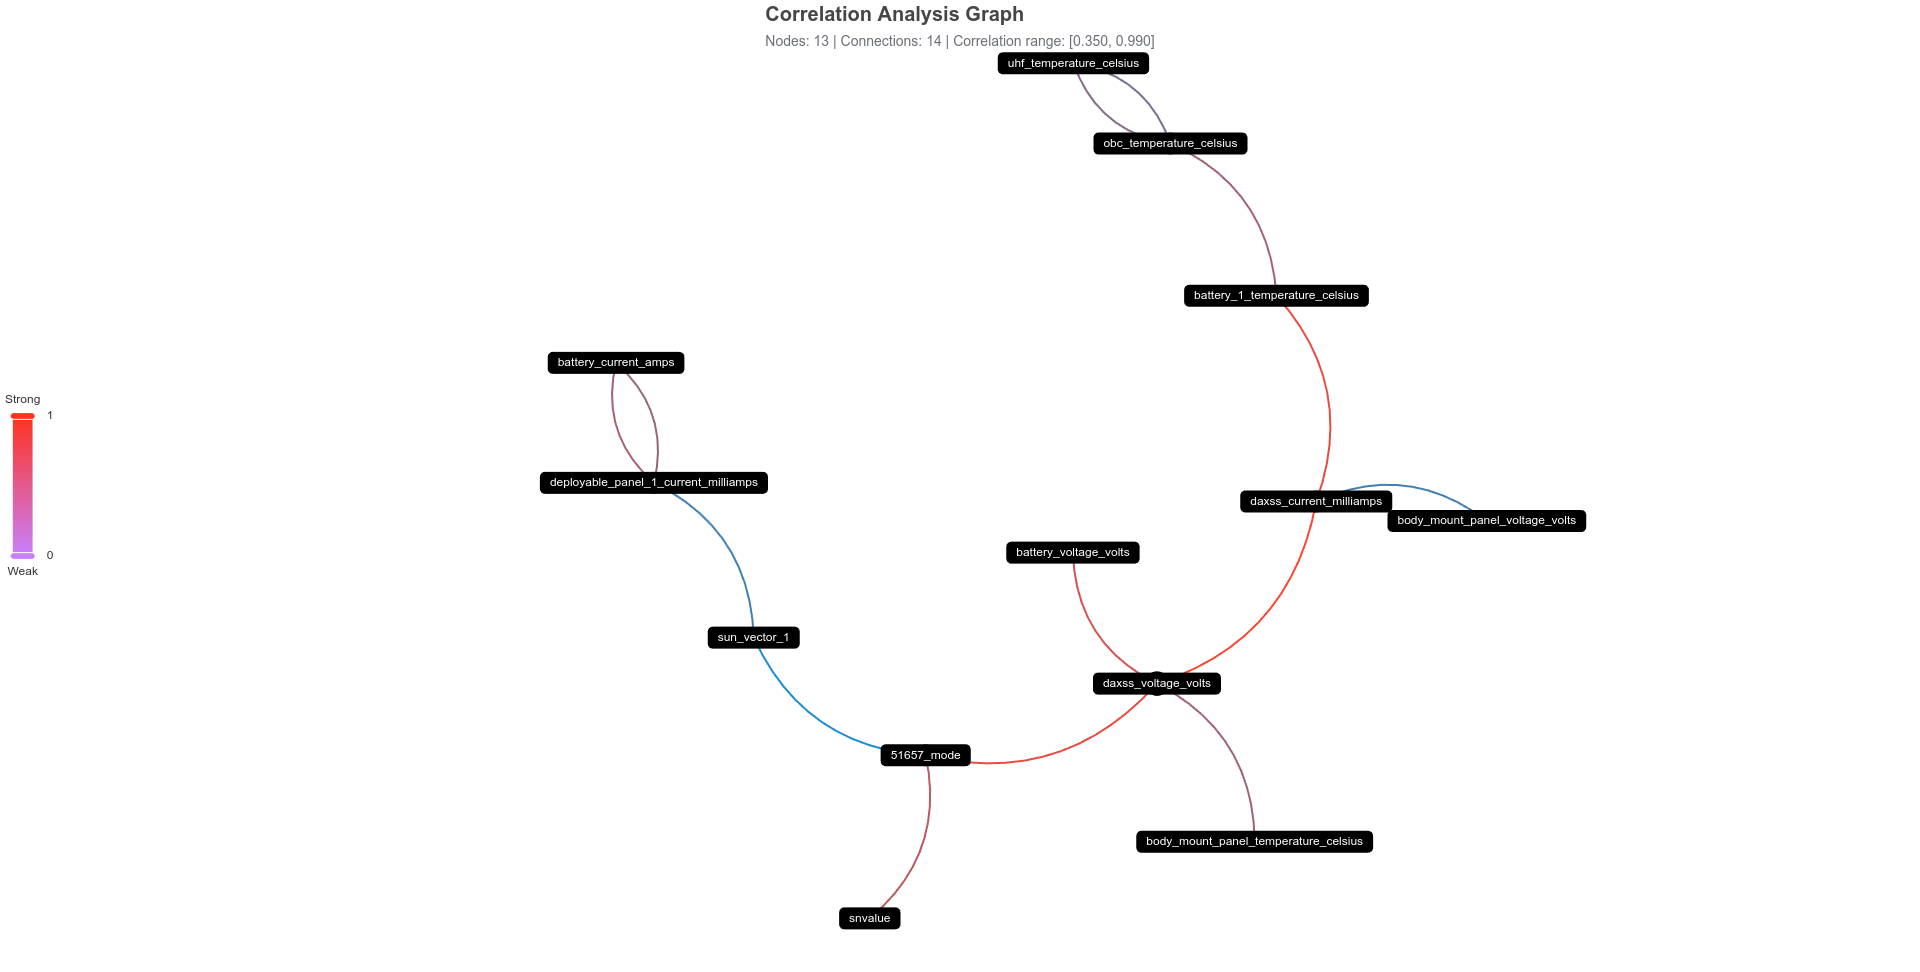
\includegraphics[width=0.95\textwidth]{sat/inspiresat_sunspot.png}
	\caption{Граф кросс-корреляций по солнечным пятнам и инженерным параметрам (INSPIRESat-1)}
	\label{fig:inspiresat_sunspot}
\end{figure}

\begin{figure}[H]
	\centering
	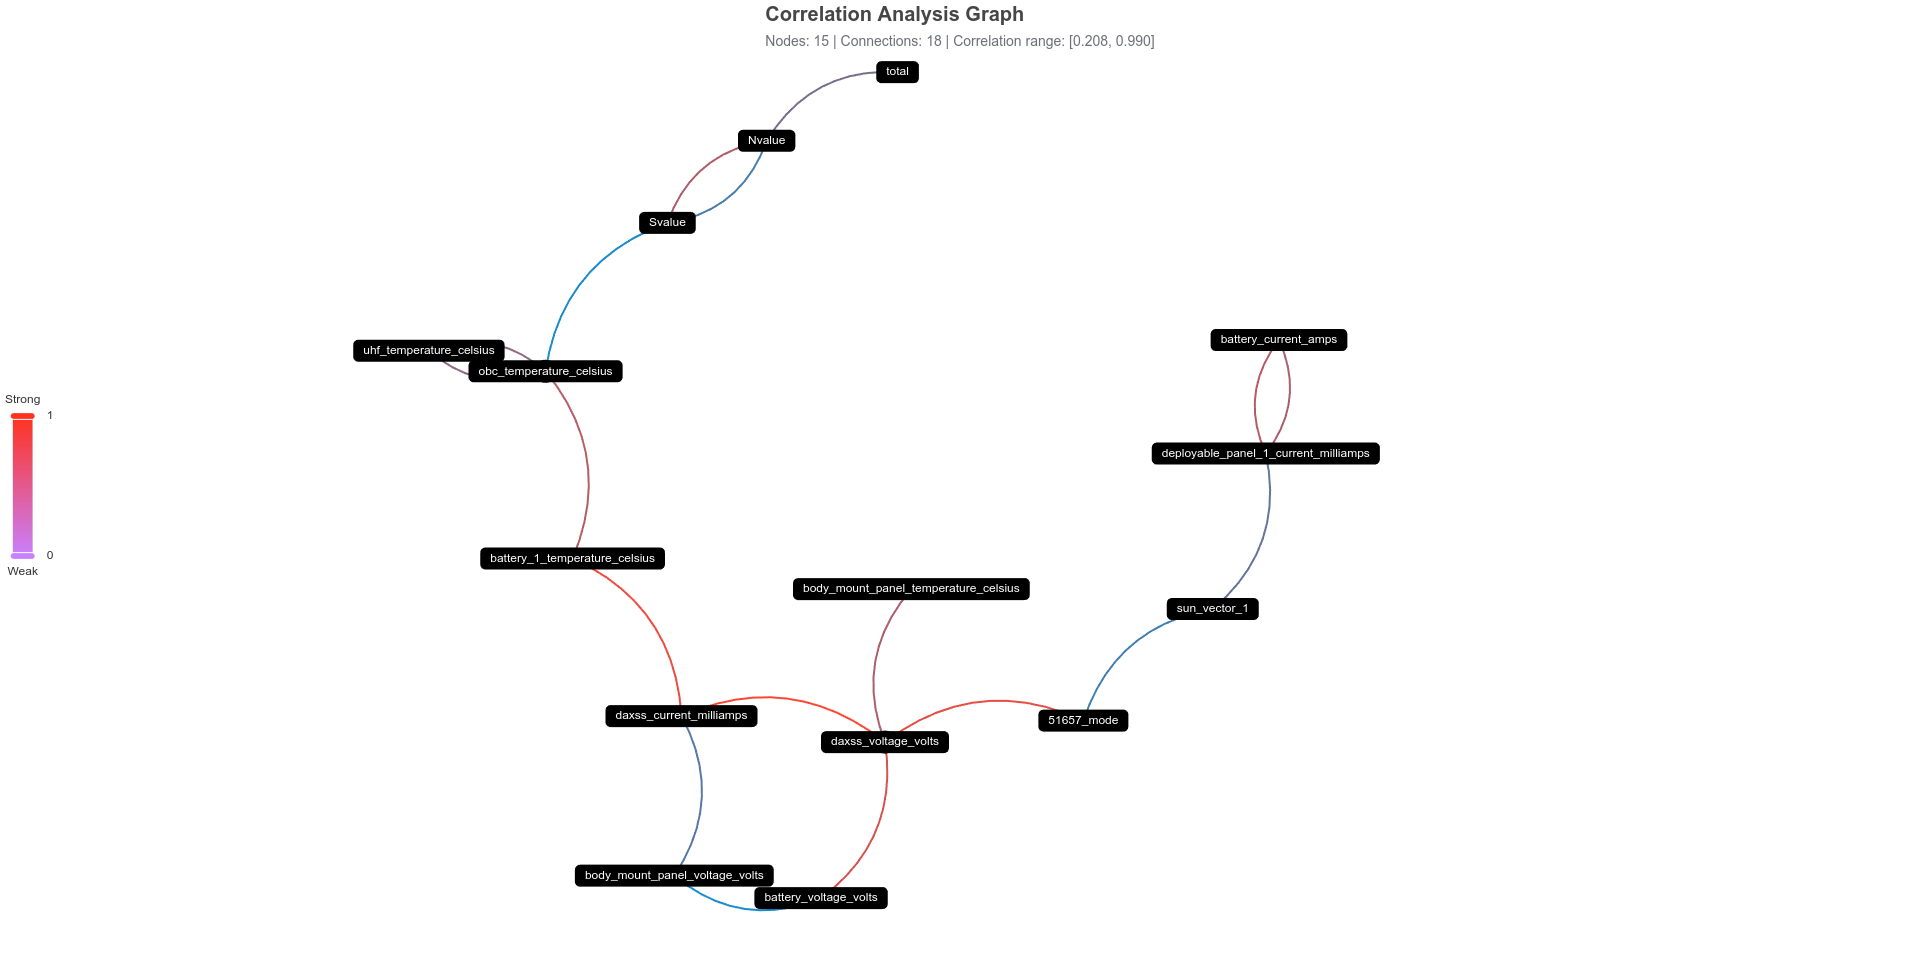
\includegraphics[width=0.95\textwidth]{sat/inspiresat_hemi.png}
	\caption{Граф кросс-корреляций по гемисферическим числам солнечных пятен (INSPIRESat-1)}
	\label{fig:inspiresat_hemi}
\end{figure}

\begin{figure}[H]
	\centering
	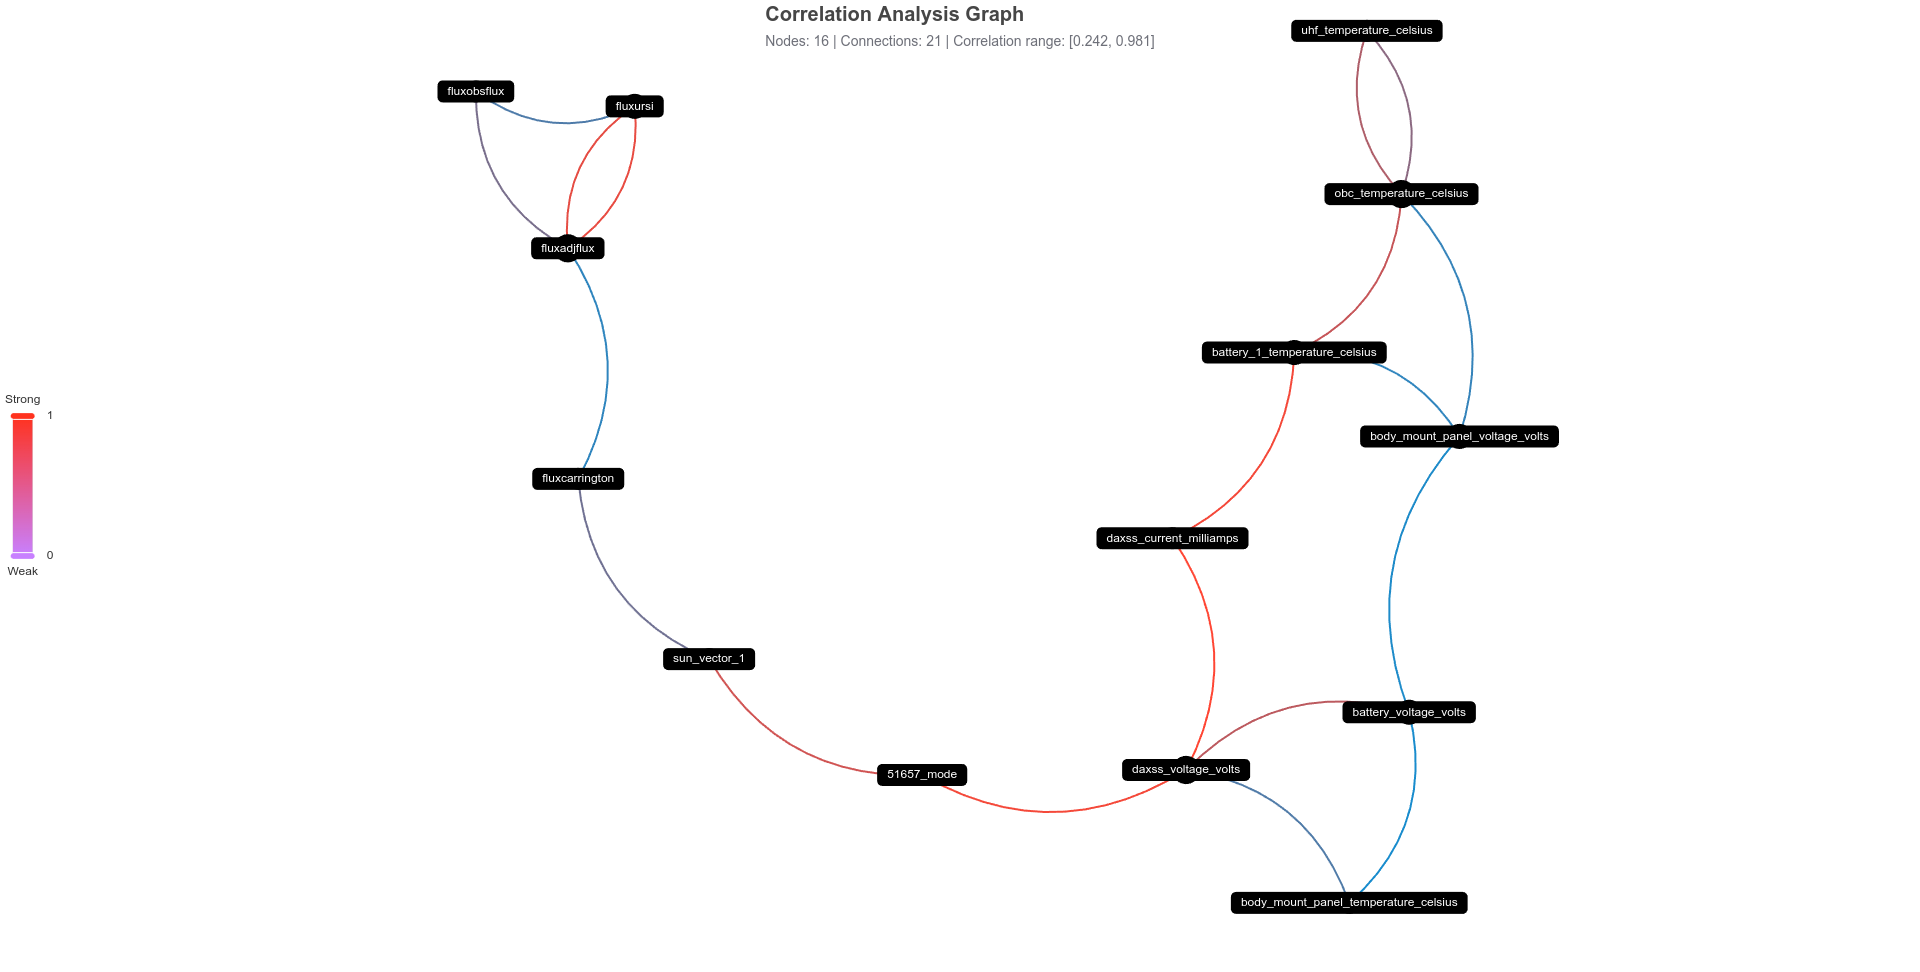
\includegraphics[width=0.95\textwidth]{sat/inspiresat_flux.png}
	\caption{Граф кросс-корреляций по солнечному радиоизлучению (INSPIRESat-1)}
	\label{fig:inspiresat_flux}
\end{figure}

\begin{figure}[H]
	\centering
	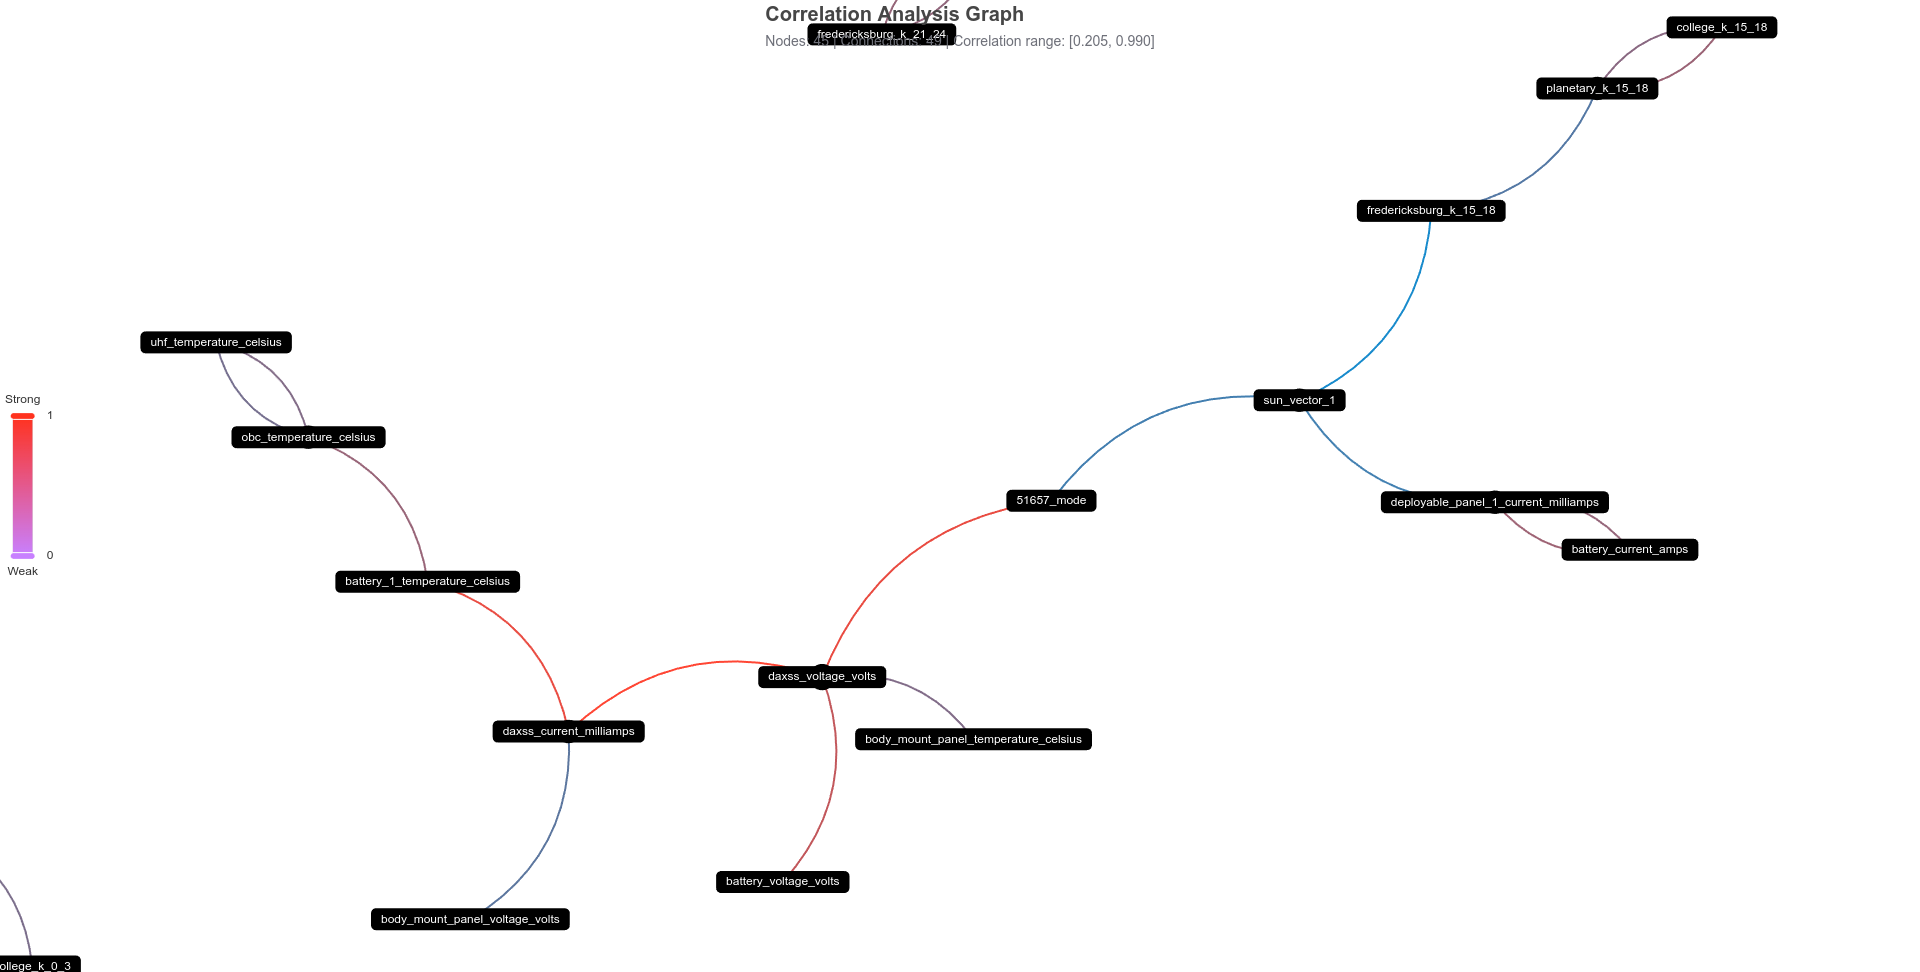
\includegraphics[width=0.95\textwidth]{sat/inspiresat_dgd.png}
	\caption{Граф кросс-корреляций по основным солнечным и геомагнитным индексам (INSPIRESat-1)}
	\label{fig:inspiresat_dgd}
\end{figure}

Анализ графов выявляет несколько ключевых особенностей взаимосвязей между
параметрами. Центральными узлами в большинстве графов являются параметры,
связанные с энергетической подсистемой и тепловым режимом спутника:
\texttt{51657\_mode}, \texttt{battery\_current\_amps},
\texttt{battery\_voltage\_volts}, \texttt{daxss\_current\_milliamps},
\texttt{daxss\_voltage\_volts}.

Особого внимания заслуживает сложная система связей между режимом работы
спутника (\texttt{51657\_mode}) и другими параметрами. Сильная корреляция
(красное ребро) между \texttt{51657\_mode} и \texttt{daxss\_voltage\_volts}
указывает на то, что режим функционирования непосредственно зависит от
энергоснабжения научной аппаратуры. При этом наблюдается средняя по силе связь
(фиолетовое ребро) между \texttt{51657\_mode} и \texttt{smvalue}, что может
свидетельствовать о переключении режимов на основе диагностических данных.

Примечательной особенностью является наличие двойных связей между
\texttt{uhf\_temperature\_celsius} и \texttt{obc\_temperature\_celsius}, что
указывает на взаимное влияние этих температурных параметров друг на друга. Это
может объясняться тепловым взаимодействием между радиокомплексом и бортовым
компьютером, расположенными в тесном пространстве спутника. Такая тепловая связь
может создавать как позитивные эффекты (поддержание рабочей температуры в
холодных условиях), так и негативные (риск перегрева при интенсивной работе
обоих компонентов)~\cite{core_inspiresat}.

Анализируя связи между солнечными параметрами и техническими характеристиками,
можно отметить неоднозначный характер влияния. С одной стороны, наблюдается
положительная корреляция между \texttt{sun\_vector\_1} и током солнечной панели
\texttt{deployable\_panel\_1\_current\_milliamps}, что ожидаемо: лучшая
ориентация на Солнце увеличивает выработку энергии. С другой стороны,
присутствуют более сложные взаимосвязи: параметр \texttt{sun\_vector\_1} имеет
связь с \texttt{fluxcarrington}, а тот, в свою очередь, коррелирует с группой
параметров солнечного излучения (\texttt{fluxadjflux}, \texttt{fluxobsflux},
\texttt{fluxursi}). Это может указывать на то, что при увеличении солнечной
активности изменяется не только энергетический баланс, но и логика ориентации
спутника, возможно, для оптимизации работы научной аппаратуры или минимизации
термических воздействий~\cite{nanosats_inspiresat}.

На графе рис.~\ref{fig:inspiresat_dgd}
заметна
слабая связь между геомагнитными индексами (\texttt{fredericksburg\_k\_15\_18},
\texttt{planetary\_k\_12\_15}, \texttt{college\_k\_15\_18}) и параметром
\texttt{sun\_vector\_1}, что может указывать на влияние геомагнитных возмущений
на систему ориентации спутника. Однако отсутствие сильных связей между
геомагнитными индексами и параметрами питания или температуры подтверждает
относительно высокую устойчивость INSPIRESat-1 к геомагнитным воздействиям.

Интересен каскадный эффект, наблюдаемый на графе
рис.~\ref{fig:inspiresat_sunspot}:
\texttt{battery\_current} $\rightarrow$
\texttt{deployable\_panel\_current} $\rightarrow$
\texttt{sun\_vector} $\rightarrow$
\texttt{daxss\_voltage} $\rightarrow$ \texttt{daxss\_current}.
Такая цепочка связей позволяет проследить комплексное влияние внешних факторов
на работу научной аппаратуры через изменение энергетического состояния и режимов
функционирования спутника.

Температурная динамика, отраженная в сильных связях между
\texttt{battery\_1\_temperature}, \texttt{obc\_temperature} и
\texttt{uhf\_temperature}, указывает на критическую важность теплового
режима для INSPIRESat-1. При этом связь между температурой и током
(\texttt{daxss\_current}) может свидетельствовать о влиянии теплового
состояния на эффективность работы научной аппаратуры. Это особенно важно для
DAXSS, чувствительность которого к тепловым воздействиям может быть
высокой~\cite{eoportal_inspiresat}.


\section{Выводы по главе}

Проведен анализ графов кросс-корреляций между телеметрическими параметрами пяти спутников различных архитектур и индексами солнечной активности с использованием Polaris ML 2.0. Установлено, что влияние космической погоды определяется архитектурными решениями: GRIFEX с rad-hard компонентами демонстрирует устойчивость и положительные корреляции между солнечной активностью и энергетическими параметрами, в то время как CubeSat на коммерческих компонентах показывают сложные нелинейные зависимости с каскадными эффектами при экстремальных событиях. Выявлены сильные корреляции внутри кластеров солнечных параметров и слабые связи с геомагнитными индексами, подтверждающие доминирование прямого солнечного излучения над геомагнитными эффектами.
